%!TEX root = ../tobias_neumann_phd_thesis.tex

\chapter{Introduction}

The information content of an organism is stored in its DNA and its functional units - genes - are transcribed into RNA that is eventually translated into proteins carrying out a specific function \citep{Crick1970CentralBiology}. The sum of all of its RNA transcripts in a cell is referred to as the transcriptome which encompasses both protein-coding transcripts and all other non-coding RNAs. Understanding the transcriptome is essential to gain insights into central biological processes such as cell differentiation, cancer development, or transcriptional regulation among others \citep{Wang2009}. The gold-standard method to investigate the transcriptome is RNA sequencing (RNA-seq): RNA sequencing couples high-throughput sequencing with subsequent computational methods for identifying and quantifying the presence of transcripts in an RNA extract \citep{Lowe2017}, with the analysis of differentially expressed genes between conditions of interest being its most popular application to date. Beyond conventional RNA-seq, the scope of RNA-seq has broadened extensively to over almost 100 distinctly derived applications\footnote{https://www.illumina.com/content/dam/illumina-marketing/documents/applications/ngs-library-prep/for-all-you-seq-rna.pdf}, further shaping our understanding of RNA biology and the transcriptome \citep{Stark2019}, such as investigating mRNA splicing \citep{Wang2008}, nascent transcription \citep{Kwak2013}, RNA-protein interaction \citep{Hafner2010}, RNA modifications \citep{Dominissini2012} or RNA structure \citep{Lucks2011}. The most recent class of these emerging profiling methods generally termed epitranscriptomics sequencing \citep{Li2016} employ chemical conversions of modified nucleotides, using them as detectable labels or anchors, to detect base modifications \citep{Schaefer2009}, map transient transcripts \citep{Schwalb2016} or track gene expression dynamics \citep{Herzog2017} and splicing kinetics \citep{Wachutka2019}. While the final readout of individual epitranscriptomics methods is quite diverse - ranging from read-counts, calling labelled reads, determining the fraction of spliced to mature read sets or calling modified sites - the one constant all methods base their results on is mapping the resulting read set against a reference. It is therefore crucial to ensure accurate and robust read-mapping to obtain meaningful and unbiased readouts in any experiment. To analyze the resulting sequencing data, a plethora of general purpose mapping tools such as STAR \citep{Dobin2013} and HISAT2 \citep{Kim2019} exist. However, for this new class of sequencing methods involving nucleotide conversions, there is a clear lack of dedicated tools which take the characteristics of such datasets into account. The current strategies to analyze such datasets center around either applying aforementioned general purpose mapping tools with all their caveats such as potential reduced mapping sensitivity due to elevated mismatch rates when it comes to handling nucleotide conversions or transferring established methods from their DNA counterpart such as Bisulfite sequencing \citep{Rieder2016} to the RNA domain. 
In this thesis, we address and comprehensively evaluate the challenges of read mapping with diverse nucleotide conversion types and rates as produced by epitranscriptomics sequencing technologies. In chapter \ref{chap:slamdunk}, we propose a method to robustly map and quantify nucleotide conversions stemming from such sequencing technologies. In a practical application, we implement it for the newly developed SLAM-seq protocol \citep{Herzog2017} which incorporates nucleotide analogs that can be read out via a chemical conversion step as mismatches in the resulting read set and effectively label RNA molecules to trace their fate over time. In chapter \ref{chap:splice_sim}, we introduce a comprehensive RNA-seq simulation framework dedicated to simulating short reads from arbitrary mixes of (partially) spliced isoforms and introducing nucleotide conversions at user configurable rates, to comprehensively and systematically benchmark and evaluate the performance and biases of general purpose and specialized mapping tools and their impact on the intermediate and final readout of epitranscriptomics experiments.

\section{Transcriptomics}
The transcriptome provides important information about cell identity and function \citep{JIMENEZCHILLARON201481} and comprises different RNA species, where \mbox{mRNAs} serve as intermediate information carrying molecules between the nucleus and the ribosome that effectively synthesises proteins, while non-coding RNAs perform other functions such as RNA splicing, DNA replication or gene regulation \citep{Lowe2017}.
Transcriptomics technologies to study an organism's transcriptome have revolutionized the field and our understanding of the transcriptome by repeated technological innovations, leading to currently two key contemporary techniques in the field: (1) microarrays - quantifying a set of predetermined sequences, and (2) RNA sequencing - capturing and sequencing all transcripts on high-throughput sequencing platforms \citep{Lowe2017}. Microarrays require prior knowledge about the organism of interest, such as an annotated genome sequence, to generate short oligomers called "probes" which are arrayed on a solid surface e.g. a glass plate \citep{Romanov2014}. Hybridisation of fluorescently labelled transcripts leads to a detectable fluorescence intensity signal at each probe location indicating the transcript abundance \citep{BarbulovicNad2006}.
Since its introduction in the late 2000s \citep{Mortazavi2008,Marioni2008}, RNA sequencing has become an indispensible, well-established and ubiquitously used technique in the field of Molecular Biology, overtaking microarrays as the dominant technique \citep{Su2014} due to its high throughput and deep and unbiased sampling of the transcriptome.

\subsection{RNA}

Ribonucleic acid (RNA) is a nucleic acid which along with deoxyribonucleic acid (DNA) encompass one of the four major macromolecules essential for life, the other three being carbohydrates, proteins and lipids. Structurally, an RNA molecule is a polymer composed of a backbone made of repeats of sugar called ribose and attached to it one of four bases: adenine (A), uracil (U), cytosine (C) or guanine (G). Unlike DNA, RNA molecules are mostly single stranded but they can have complex structures like helices and bridges induced by self-complementary base pairing \citep{AlbertsB2002MolecularEdition}. There are different types of RNA in eukaryotes with the three most well-known types being messenger RNA (mRNA), ribosomal RNA (rRNA) and transfer RNA (tRNA) which are crucial for protein synthesis. Messenger RNAs are single stranded RNA molecules which carry the genetic information encoded in DNA in the nucleus to the protein synthesis machinery - the ribosome - in the cytoplasm. Ribosomes are composed of proteins and rRNA molecules which are protein non-coding RNAs and the most abundant type of RNAs in a cell. rRNAs play a crucial role during the synthesis of the chain of amino acids encoded in mRNA by catalyzing the formation of peptide bonds and providing the structural scaffold for the ribosome. The third type of RNAs are tRNAs - small RNA molecules which serve as adaptors physically linking the messenger RNA and the amino acid sequence of the proteins via bringing amino acids to the ribosomes \citep{Solomon2007}.

\begin{figure}
	 \centering
	 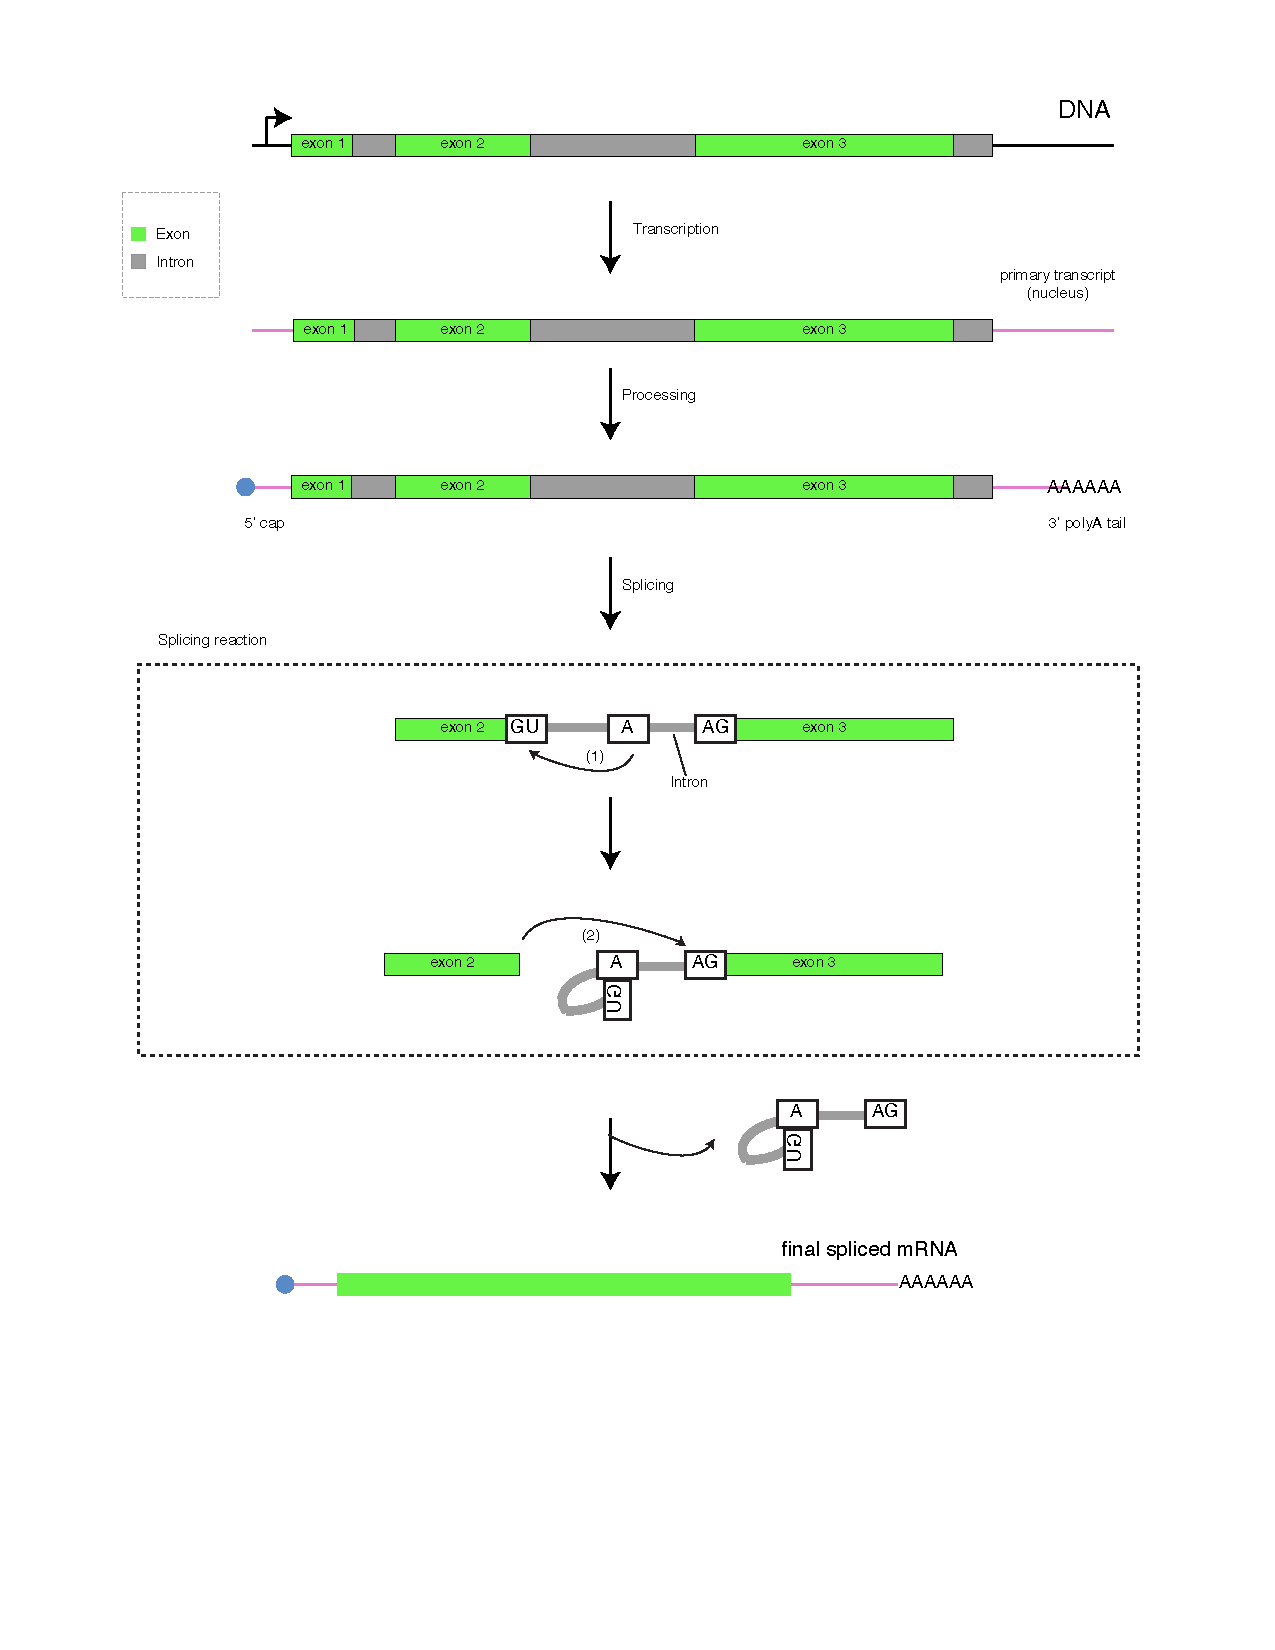
\includegraphics[width=1\linewidth]{img/chapter1/rna}
	  \caption[RNA processing]{\textbf{RNA processing.} Transcripts are synthesized during transcription from a continuous genomic DNA template to form a primary RNA transcript and are processed co-transcriptionally by adding a cap in the 5' and a poly-A tail at the 3' end of the transcript. A complementary processing step is the removal of non-coding intron sequences via splicing to form the final mature mRNA transcript.}
	 \label{fig:rna}
\end{figure}

The RNA molecules are synthesized using DNA as template in a process called transcription and the newly synthesized RNA molecules are called transcripts. The synthesis is mediated by RNA polymerases via the addition of ribonucleotides (ribose sugar and a base) in 5' to 3' direction. The transcription initiation is directed by DNA sequences called promoters \citep{Haberle2018}. Most transcripts must be processed before becoming fully functional. For newly synthesized mRNA transcripts called pre-mRNA this processing consists of 3 steps (see Figure \ref{fig:rna}): capping, polyadenylation, and splicing \citep{AlbertsB2002MolecularEdition}. Capping is the addition of 7-methylguanylate to the 5' end of mRNA transcript and is important for protecting the transcript from exonuclease activity and for positioning the mRNA in the preinitiation complex during protein synthesis \citep{Darnell1979,Shatkin1976,Filipowicz1976}. Polyadenylation is the addition of adenylate residues as poly-A tail at the 3' end of the transcript \citep{Wahle1999}. The polyA tail protects the mRNA molecules from exonucleolytic degradation \citep{Wu2012}. Splicing is the removal of protein noncoding sequences, derived from the DNA template, from the pre-mRNA to form a functional mRNA. These noncoding sequences are known as introns and the protein coding sequences are called exons. Most introns have a donor site sequence GU at their 5' ends and an acceptor AG sequence at their 3' ends \citep{Moore1993}. During splicing, the guanyl residue at the 5' end of the intron is linked by a 2' to 5' phosphodiester linkage to an adenylate residue called a branch site within the intron. The result is a lariat (loop) structure and the release of the 3' end of the first exon \citep{Wachtel2009}. The 3' end of the intron is spliced by a ribonucleoprotein complex known as spliceosome, which releases the loop and frees the 5' end of the second exon \citep{doi:10.1146/annurev.bi.65.070196.002055}. The exons are then joined together forming the final functional mRNA transcript which is then transported to the cytoplasm to initiate protein synthesis.

\paragraph{RNA-seq}

The quantification of RNA transcript abundances across different biological conditions is done via a next generation sequencing technology called RNA sequencing or RNA-seq  \citep{Nagalakshmi2008}. The general steps in an RNA-seq protocol include (1) isolation of RNA, (2) enrichment of RNA species via selection or depletion, (3) synthesis of DNA via reverse transcription of RNA to cDNA, (4) library preparation including fragmentation, size selection, barcoding, amplification and sequencing \citep{Griffith2015,Wang2009}.
Although canonical RNA-seq analysis is crucial for probing RNA transcript abundance and variation across different conditions, it has two key limitations: (1) it provides only a static view or a  "snapshot" of the transcriptome without direct information on RNA dynamics and (2) it does not allow the study of post-transcriptional modifications and interactions with RNA-binding proteins \citep{Kleiner2021}. These limitations led to the development of different modifications of the canonical RNA-seq workflow to allow the study of RNA dynamics, RNA posttranscriptional modifications and RNA binding partners.

\subsection{Epitranscriptomics}

The term epitranscriptome encompasses the large variety of chemical modifications affecting RNA transcripts. More than 170 distinct modifications have been identified and characterized up to date \citep{Boccaletto2018} in all known species of RNA (both coding and noncoding RNA transcripts) with the ribosomal RNA (rRNA) and transfer (tRNA) being the most heavily modified. They can be introduced as posttranscriptional modification and are crucial for the normal development and play a key role in the regulation of the gene expression programs and adaptation to changes in the environment \citep{Frye2018,Roundtree2017}.  Modifications of all RNA species have been linked to various diseases like cancer, the full pathology of which has yet to be elucidated \citep{Barbieri2020}.  The deposition, removal and regulation of these modifications is done by proteins which in general can be split in 3 groups: \textit{writers} (introducing the chemical modification), \textit{readers} (specialized domain containing proteins which identify and interpret modifications) and \textit{erasers} (proteins removing the modification) \citep{Nie2020}. \\
From all RNA species, tRNAs have the largest number and chemical diversity of modifications. They range from base modifications (isomerization, methylations) and ribose methylations to elaborate ring structures. tRNA modifications are important for the efficiency and fidelity of decoding and folding of proteins, for cellular stability and localization, and are shown to be reversibly deposited in response to stress, thus highly important for  biological regulation \citep{Pan2018}. \\
The most common rRNA modifications in eukaryotes are 2'-O-methylation of the ribose and isomerization of uridine to pseudouridine ($\Psi$) \citep{Sloan2017}. Without these modifications, rRNA biogenesis is blocked. Most rRNA modifications occur in or close to functionally important sites and facilitate efficient and accurate protein synthesis \citep{Delaunay2019}. Defects in rRNA modifications have been linked to dyskeratosis congenita, a human disease that affects pseudouridylation. \\
mRNA modifications affect protein production by modulating splicing, translation, and decay rates. mRNAs contain numerous modified nucleosides like base isomerization (pseudouridine ($\Psi$)); methylation of the bases (m$^6$A, m$^1$A, and m$^5$C); methylation of the ribose (2'O-methylation (Nm, m$^6$A$_m$)); pathological oxidations (8-Oxo-7,8-dihydroguanosine) and many more \citep{Roundtree2017,Boo2020}. In addition to posttranscriptional modifications, chemical modifications can be incorporated into RNA molecules via metabolic labeling approaches which can be used to e.g. assess the kinetics of RNA biogenesis and degradation. With mRNAs being the most popular and broadly studied RNA, we will focus in this section on selected relevant types of physiological modifications in mRNAs and the approaches for their subsequent detection (see Figure \ref{fig:base_modifications}).
 
 \begin{figure}
	 \centering
	 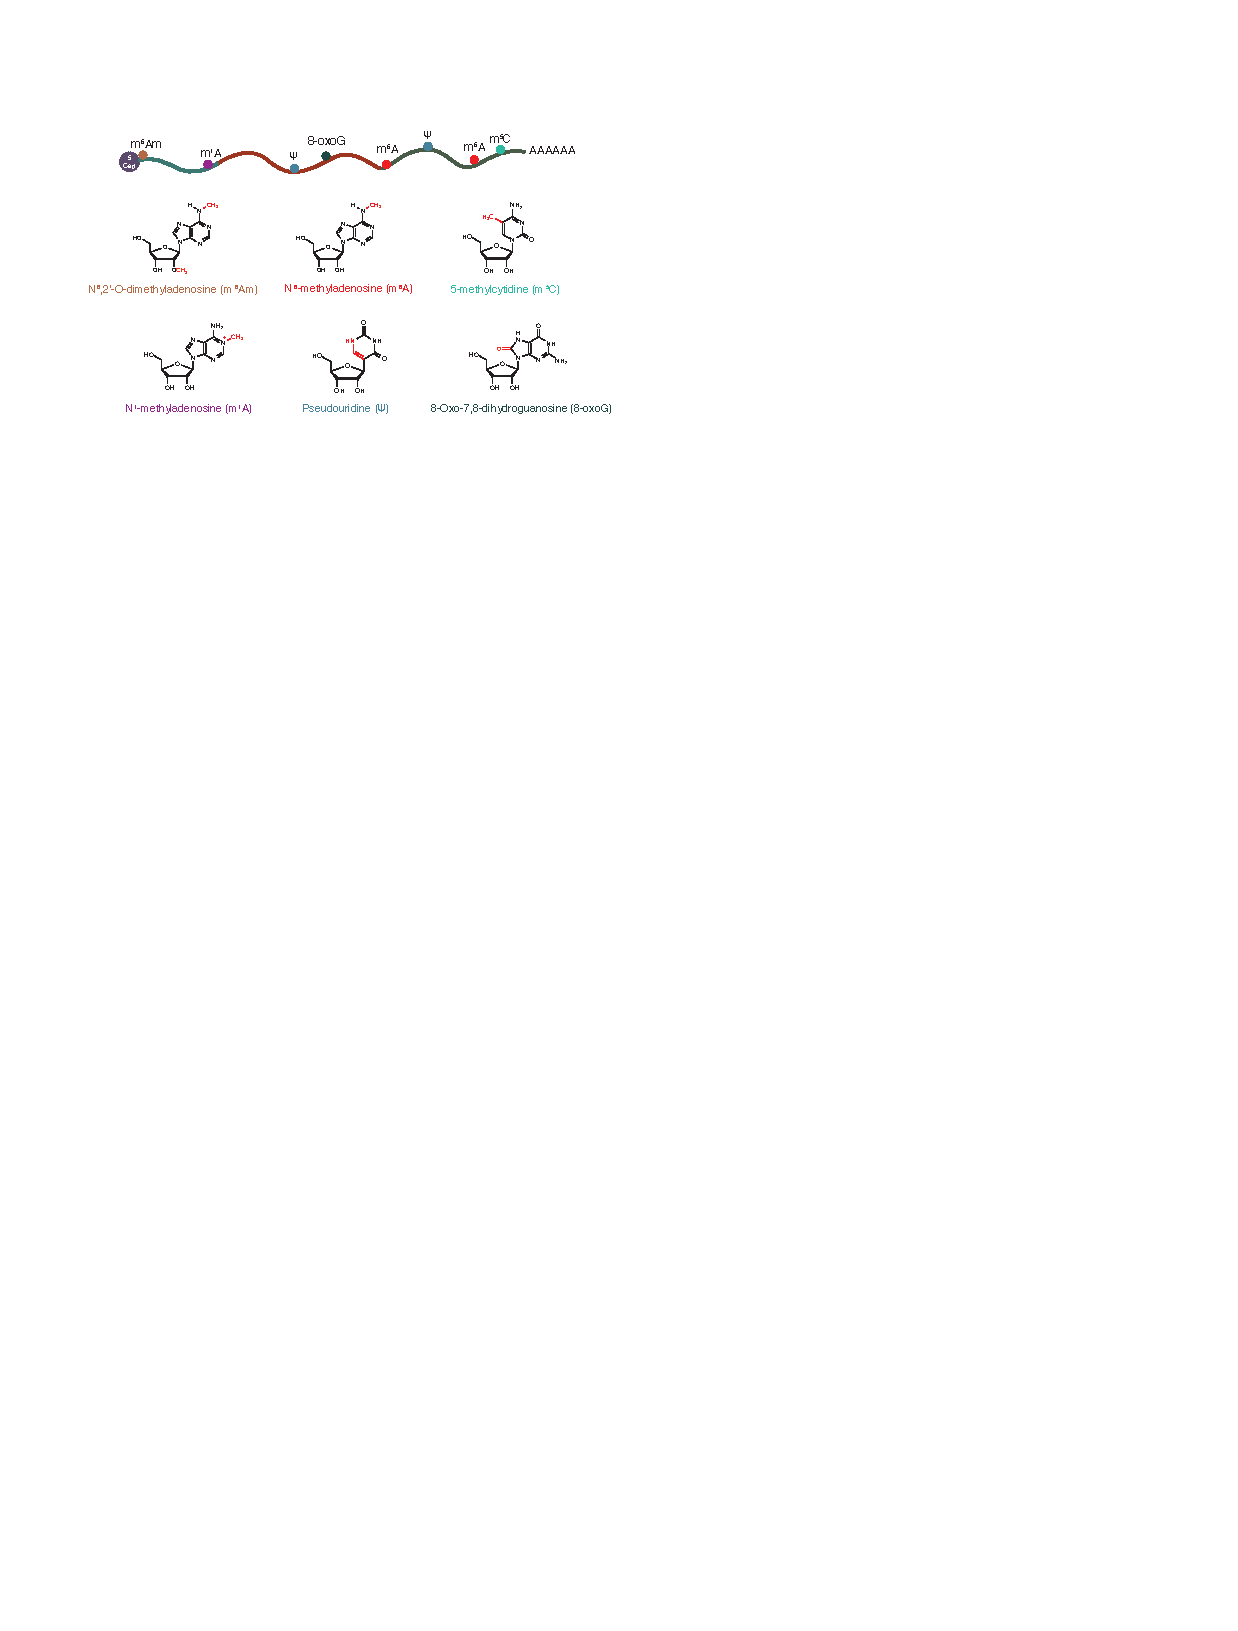
\includegraphics[width=1\linewidth]{img/chapter1/base_modifications}
	  \caption[Relevant base modifications in RNA]{\textbf{Relevant base modifications in RNA.} Schematics of relevant and well-studied RNA modifications and exemplary deposition along an RNA transcript discussed in this section (modified from \citeauthor{Li2016} \citep{Li2016})}
	 \label{fig:base_modifications}
\end{figure}
 
 \paragraph{5-methylcytosine (m$^5$C):} Methylation at the 5 position of cytosine in mRNA was discovered more than 40 years ago \citep{Desrosiers1974,Dubin1975}. This modification is identified using various sequencing derived methods like bisulfite sequencing \citep{Schaefer2009}, m5C RNA immunoprecipitation sequencing (m5C-RIP-seq) \citep{Edelheit2013}, 5-AZAcytidine-mediated RNA immunoprecipitation sequencing (Aza-IP-seq) \citep{Khoddami2014} and methylation-individual nucleotide resolution crosslinking immunoprecipitation sequencing (miCLIP-seq) \citep{Hussain2013}. m$^5$C sites were mapped in human mRNA and lncRNAs, particulary enriched in untranslated regions, and were found to be recognized and specifically exported from the nucleus  \citep{Yang2017}. This modification is important for mRNA translation \citep{Cui2017}, transport \citep{Yang2017} and stability \citep{Cui2017,Yang2019}.
 
\paragraph{N6-methyladenosine (m$^6$A):} m$^6$A is the methylation of the N6-position of adenosine and is the most abundant and well-studied modification on eukaryotic mRNA \citep{Dominissini2012,Meyer2012}. This modification is important for regulating gene expression by attenuating  transcription, pre-mRNA splicing, mRNA export, mRNA stability, and translation, thereby influencing cellular processes ranging from cell self-renewal, differentiation, invasion to apoptosis \citep{He2019,Nachtergaele2018}. m$^6$A is installed by m$^6$A methyltransferases, removed by m$^6$A demethylases and recognized by various reader proteins \citep{Zaccara2019}. Alteration of m$^6$A levels participates in cancer pathogenesis and development via regulating expression of tumor-related genes \citep{Luo2018,Chang2019,He2019}. There are various approaches for detection of this modification with historically first antibody-based mapping of m$^6$A via m6A-seq \citep{Dominissini2012} or MeRIP-seq \citep{Meyer2012}. The antibody reacts with other methyl RNA species \citep{Linder2015,Mauer2017} leading to the development of other approaches -  UV cross-linking and immunoprecipitation (CLIP) m6A-CLIP \citep{Ke2015},  miCLIP/miCLIP2 methods \citep{Linder2015,Geula2015,Koertel2021} and photo-crosslinking-assisted m6A sequencing PA-m6A-seq \citep{Chen2015}. Antibody independent approaches include MAZTER-Seq \citep{GarciaCampos2019} and m6A-REF-seq \citep{Chen2022}, metabolic and enzymatic labeling via DART-seq \citep{Meyer2019}, m6A-SEAL-seq \citep{Wang2020}, via identifying the binding sites of writers with irCLASH \citep{Song2020} or via direct RNA sequencing with Oxford Nanopore Technologies with xPore \citep{Pratanwanich2021}.
  
\paragraph{Pseudouridine ($\Psi$):} $\Psi$ is the isomerization of the uridine base and the most common modification in cellular RNA, recently found in hundreds of human and yeast mRNA species \citep{Carlile2014}.  The endogenous functions of pseudouridine in mRNA are largely unknown, although $\Psi$ is dynamically deposited in response to stress and known to affect the secondary structure of RNA with recent studies suggesting that this modification is important for splicing efficiency \citep{Martinez2022}. Pseudouridine is detected genome-wide using PseudoU-seq \citep{Carlile2014}, $\Psi$-seq \citep{Schwartz2014} and via chemical labeling and pull-down methods (CeU-seq) \citep{Li2015}. 

\paragraph{N1-methyladenosine (m$^1$A):} Methylation at the N1 position of adenosine generates a positively charged base which can dramatically alter protein-RNA interactions and RNA secondary structures through electrostatic effects. m$^1$A maps uniquely to positions near the translation start site and first splice site in coding transcripts and can be deposited as stress response, correlating with upregulation of translation in general \citep{Dominissini2016,Li2016a}. m$^1$A blocks Watson-Crick base pairing and thus most reverse transcription which is used for its detection \citep{Motorin2007}. Partial read-through of m$^1$A could create mutations that mark the modification sites. However, mutations could be severely underrepresented during library preparation due to abortive reverse transcription at or adjacent to the m$^1$A site or poor amplification of short ligation products \citep{Hauenschild2015}. 

\paragraph{Ribose methylation:} Methylation of the ribose 2' hydroxyl exists at the second and third nucleotide in many mRNAs \citep{Schibler1977}. The 2' hydroxyl group  participates in contacts forming higher order RNA structures, thus methylation can impact RNA-protein interactions and RNA secondary structures. 2'-O-methylation (2'-OMe or Nm) sites in abundant RNA species such as rRNA have been mapped taking advantage of its higher resistance to alkaline-mediated hydrolysis compared to unmodified nucleosides \citep{Marchand2016}. A new approach (Nm-seq) based on ribose sensitivity to periodate cleavage allows for enrichment of 2'-OMe in low abundant RNA species such as mRNAs, providing a highly sensitive single-base method for detection \citep{Dai2017}.

\paragraph{8-Oxo-7,8-dihydroguanosine (8-oxoG):} Reactive oxygen species (ROS) like superoxide, hydroxyl radicals, and hydrogen peroxide can be byproducts of the normal oxygen metabolism or generated by environmental stress \citep{Cadet2013}. ROS can oxidize RNA bases and generate numerous forms of oxidized RNAs \citep{Yan2019,Cadet2013}. These oxidized bases include 8-oxoG, 8-oxo-7,8-dihydroadenosine, 5-hydroxyuridine, 5-hydroxycytidine, and cytosine glycol.  Among these forms, 8-oxoG (an oxidized form of the guanine base) is the most abundant within mammalian cells, and its accumulation is associated with many neurodegenerative diseases \citep{Nunomura2017,Poulsen2012}. \\

In summary, while the initial mode of detection for the discussed base modifications started off quite diverse, most subsequent detection efforts have converged to derivatives of RNA-sequencing protocols due to their versatility and throughput.

\subsection{Metabolic labelling}

 \begin{figure}
	 \centering
	 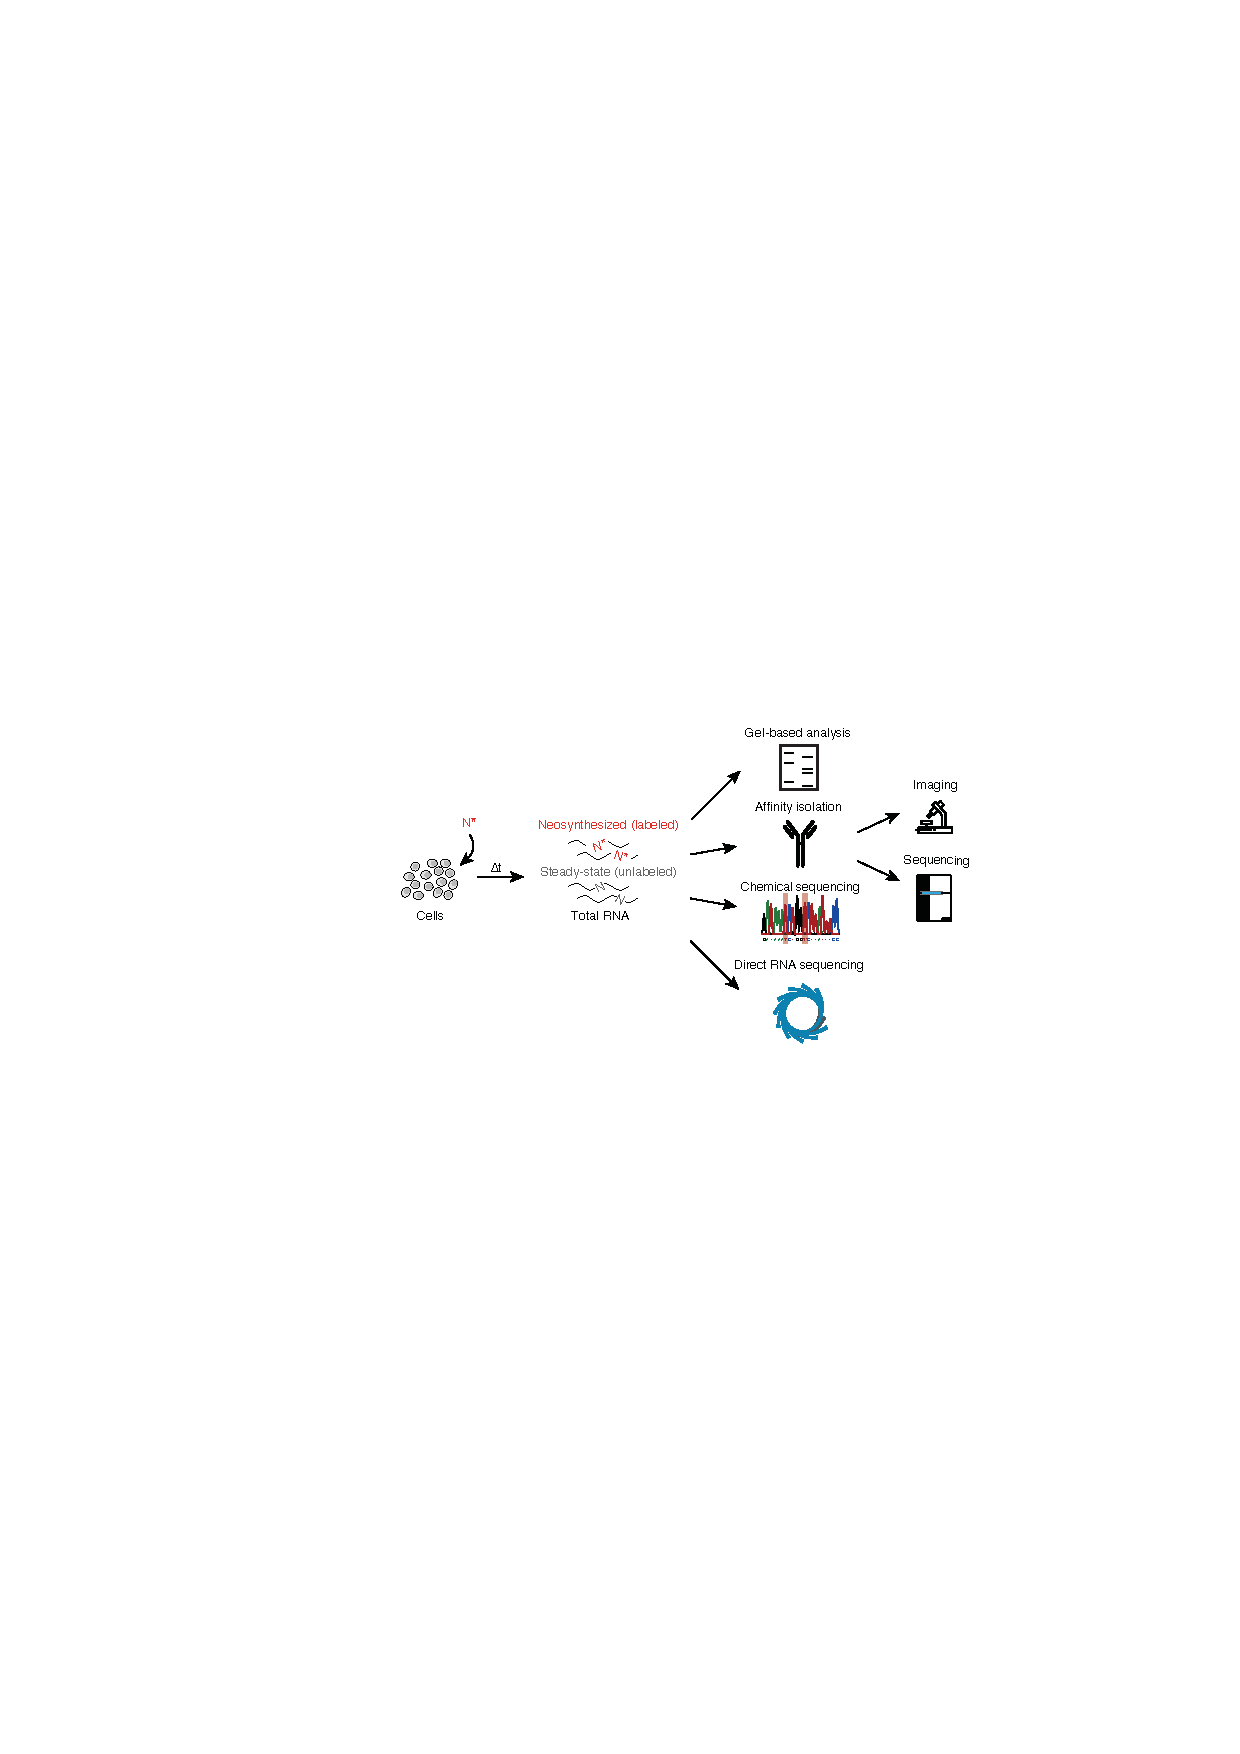
\includegraphics[width=0.9\linewidth]{img/chapter1/metabolic_labelling}
	  \caption[Metabolic labelling outline]{\textbf{Metabolic labelling outline.} Chemically modified ribonucleosides (N$^{*}$ in the schematics) are supplied to the cell and are metabolized and incorporated into newly synthesized RNA molecules by its native transcriptional machinery. Such metabolically labelled RNA molecules can be enriched for and detected via various sequencing and visualization approaches discussed in this section to probe for RNA turnover, splicing kinetics, subcellular location and other features (modified from \citeauthor{Herzog2017} \citep{Herzog2017}).}
	 \label{fig:metabolic_labelling}
\end{figure}

Metabolic labeling describes the approach where the endogenous synthesis and modification machinery of living cells is used to incorporate exogenous compounds which are then used to detect or affinity tag biomolecules. It has been applied to a variety of biomolecules in order to study their synthesis and turnover, subcellular localization, interaction partners, and other features \citep{Kleiner2021}. RNA metabolic labeling with chemically modified ribonucleosides has been applied to study transcriptome dynamics through RNA sequencing or to investigate biochemical interactions between RNA and associated RNA-binding proteins that occur within the cell. RNA-protein interactions can be mapped transcriptome-wide using crosslinking and immunoprecipitation combined with high-throughput sequencing (CLIP-seq or HITS-CLIP) \citep{Nechay2020}. These studies are critical for characterizing  RNA targets of an individual RNA binding protein, and thus reveal insights into its biological role. There are several approaches to detect these chemically modified ribonucleosides which are outlined in this section and outlined in Figure \ref{fig:metabolic_labelling}.

\paragraph{Nucleoside detection via autoradiography ($^3$H-uridine):}

Historically, the first approach to study RNA kinetics was the labelling of RNA molecules via the incorporation of a radioisotope. Here, detection of radioactively labeled RNA is achieved via gel electrophoresis and  autoradiography (gel-based assays).  One frequently used isotope is $^3$H-uridine  which was found to efficiently label and cause minimal perturbation to the native nucleotide structure \citep{Rovera1970}. Radioisotope labeling requires laborious work with radioactivity and is not compatible with next generation sequencing workflows, therefore making it a less popular method of choice nowadays.

\paragraph{Nucleoside detection via affinity isolation:}

Suitable antibodies were developed for the detection of several nucleosides that allow for isolation via antibody or streptavidin affinity selection and subsequent RNA-sequencing of the isolated population or detection via fluorescence microscopy on fixed cells.
 5-Bromouridine (BrUrd, 5BrU, br5Urd) is a halogen-containing uridine derivative with a C5 bromo modification \citep{Haider1997}. BrU can be incorporated into RNA over a long period of time  with minimal cell toxicity \citep{Tani2012}. It is detected and affinity isolated using a BrU-specific monoclonal antibody \citep{Halicka2000}. NGS sequencing, utilizing RNA labeling with BrU, has been applied to measure RNA stability transcriptome-wide via bromouridine pulse-chase and sequencing (BruChase-seq) \citep{Paulsen2013} or bromouridine immunoprecipitation chase-deep sequencing analysis (BRIC-seq) \citep{Tani2012}. BrU labeling is  used  to measure nascent transcription and therefore allows the investigation of transcription initiation and elongation via Global run-on sequencing (GRO-seq) \citep{Core2008}. Limitations of BrU-labelling are the requirement for high amounts of starting material and that it does not provide single-base resolution (the resolution depends on fragment size). Moreover, the level of noise, especially when analyzing low-abundance modifications, may lead to higher false detection rates, resulting from non-specific binding of RNA fragments to the beads used for enrichment. False site detection may also result from cross-reactivity of the antibody with other modifications. Another limitation of this approach is that it is blind to modification stoichiometry as well as to splice variants.\\
5-ethynyluridine (EU) is an alkyne containing uracil derivative which is rapidly taken up by the cells  and incorporated into transcribed RNAs. Short term EU treatments do not seem to have a negative effect on normal cell processes, but longer treatments impact cell growth. After incorporation, EU can be detected via the Cu(I)-catalyzed alkyne-azide cycloaddition (CuAAC) reaction also known as "click" chemistry \citep{Jao2008,Paredes2011}. Initially, EU labeled RNA was detected in fixed cells by fluorescence microscopy using Cu-catalyzed azide-alkyne cycloaddition (CuACC) with an azide-conjugated fluorophore reaction \citep{Jao2008}. Alternatively, CuACC labeling with azide-conjugated biotin can be performed on purified RNA followed by streptavidin affinity selection to isolate the EU-labeled RNA for RNA-seq analysis. The use of CuAAC on purified RNA is challenging due to Cu(I)-mediated RNA degradation, and CuAAC is toxic to living cells, thus the click chemistry is performed \textit{in situ} \citep{Paredes2011}. In addition, EU is significantly more expensive compared to other labeling reagents.  Several alkyne-containing ribonucleoside alternatives have been shown to be suitable for RNA metabolic labelling \citep{Curanovic2013,Grammel2012,Qu2013}. \\
An alternative to the CuAAC is the Cu-free strain-promoted azide-alkyne cycyloaddition (SPAAC) reaction which is significantly milder than CuAAC chemistry and can be used in live cells \citep{Baskin2007,Nainar2016}. 

\paragraph{Nucleoside detection via chemical sequencing:}

One of the most versatile metabolic labels is the modified nucleoside 4-thiouridine (4-SU) \citep{Kleiner2021}. 4-thiouridine is a naturally occurring uridine derivative and is readily taken-up by the nucleotide salvage pathway and  incorporated in the place of native uridine residues \citep{Parish1968,Melvin1978}. In addition, in cells that express the uracil phosphoribosyltransferase (UPRT) enzyme, the 4-thiouracil nucleobase can be used for labeling \citep{Cleary2005}. 4-SU-labeled RNA can be subjected to further chemical treatments like alkylation, disulfide formation, and oxidative-nucleophilic aromatic substitution. These treatments are used by emerging technologies to distinguish newly synthesized 4-SU-containing RNA from unmodified RNA to measure RNA turnover rates \citep{Herzog2017,Riml2017,Schofield2018,Fuchs2014,Schwalb2016,Rabani2011}. The identification of the newly synthesized metabolically labeled RNA is done via two main approaches: (1) affinity isolation or (2) mutational analysis of chemically altered 4-SU residues.  Affinity-based enrichment approaches offer higher sensitivity, which is important when metabolic labeling is performed over short periods of time, but they are associated with high inherent variability. That is why the second category of approaches provides considerable advantages. In this group are methods such as SLAM-seq \citep{Herzog2017}, TimeLapse-seq \citep{Schofield2018} and TUC-seq \citep{Riml2017}. In all 3 approaches, a T to C mutation indicates the position of the incorporated 4-SU. \\
In addition to metabolic labeling, 4-SU is broadly used in different approaches for identifying RNA interacting proteins. An example of such methods is the PAR-CLIP approach \citep{Hafner2010}, where RNA is metabolically labeled,  subjected to crosslinking, immunoprecipitated and sequenced. Compared to other approaches, 4-SU crosslinking gives a higher yield of RNA-protein crosslinking, can be more confidently distinguished from nonspecific background contamination and mapped at near nucleotide resolution because of characteristic T to C mutations occurring at the site of RNA-protein binding. Another application of 4-SU-induced protein-RNA crosslinking is to characterize the complement of RNA binding proteins in a particular sample. This method is termed "RNA interactome capture" and involves RNA-protein enrichment through denaturing antisense oligo-dT pulldown and mass spectrometry-based proteomics after metabolic labeling and in-cell crosslinking with 4-SU \citep{Castello2012}. Related approaches for studying RNA-binding proteins relying upon 4-SU-mediated protein-RNA crosslinking have also been described \citep{He2016,Shchepachev2019,Huang2018,Trendel2019,Queiroz2019}.
Alternatives to 4-SU are for example 6-thioguanosine (6-SG) that can be incorporated instead of guanine and used similarly to 4-SU for metabolic labeling and detection of RNA turnover and RNA-binding proteins \citep{Gasser2020,Hafner2010}. The incorporated 6-SG can be chemically converted to 2-aminoadenosine leading to G to A mutations and was used in pulse-chase experiments in combination with 4-SU to measure RNA-decay rates with higher accuracy \citep{Gasser2020}. Unlike 4-SU, higher concentrations of 6-SG and prolonged labeling are toxic for the cells \citep{Woodford1988}. \\
Another alternative is the metabolic incorporation of N6-allyladenosine which happens at much lower rate than that of pyrimidine nucleosides like 4-SU, and has precluded the widespread use of this derivative \citep{Shu2017}.

\paragraph{Direct RNA sequencing by Nanopore sequencing:}

 Instead of chemical recoding or affinity enrichment, a recent strategy for measuring RNA turnover relies upon direct RNA sequencing using Nanopore sequencing to detect metabolic labeling events. In this approach, known as Nano-ID, the modified nucleoside is detected directly in RNA through perturbations in the Nanopore ioinic current signal \citep{Maier2020}.
 
\section{Analysis of RNA sequencing data}

RNA-seq experiments typically generate a large volume ($10^6$ - $10^9$) of raw sequencing reads stemming from RNA transcripts, where each read represents a tiny piece of the full complement of RNA molecules in an experiment \citep{Lowe2017}. As each read carries only little information \citep{Canzar2015}, this data has to be processed and aggregated to obtain a faithful representation of the RNA snapshot for the researchers to interpret. Typically, the read sequence itself is used to identify the transcript the read originated from and the overall number of reads stemming from a given transcript correlate with the abundance of this transcript in the total RNA pool. The process to obtain a biological readout from the raw sequencing read set is highly dependent on the chosen method and experimental design as illustrated in Figure \ref{fig:rna_seq_processing}, but the one thing in common is the initial step of assigning the raw reads to their sequence of origin. If a reference is available, the reads can be assigned via reference-based read mapping which has been well established over the last years \citep{Haas2010}. 

\begin{figure}
	 \centering
	 \includegraphics[width=1\linewidth]{img/chapter1/rna_seq_processing-block_diagram}
	  \caption[Alternative RNA-seq data processing workflows]{\textbf{Alternative RNA-seq data processing workflows.} While there are a wide variety of RNA-seq derived methods and processing steps available (a subset illustrated in the boxed steps on the right-hand side) which all require specialized post-processing steps (white boxes) and result in distinct outputs (purple boxes) and readouts, all processing steps have their foundation in accurate transcript origin identification of the raw sequencing read set (green cylinder) via reference-based read mapping or \textit{de-novo} transcript assembly (blue boxes).}
	 \label{fig:rna_seq_processing}
\end{figure}

However, if a reference genomic sequence is not available, is gapped, highly fragmented or substantially altered as in cancer cells, transcripts have to be reconstructed \textit{de-novo} from the read set by comparing reads and collapsing them into larger sequences if they overlap sufficiently \citep{Grabherr2011}. These larger sequences called contigs represent individual transcripts from the total sequenced RNA pool in an ideal scenario. To circumvent the computationally intensive task of having to compare all reads against each other, sophisticated data structures like de-bruijn graphs \citep{Pevzner2001} and algorithms have been developed to optimise the process of \textit{de-novo} assembly \citep{Schatz2010}. While in principal this approach results in an unbiased reconstruction of the transcriptome of a sequenced sample, there are numerous challenges to \textit{de-novo} assembly approaches: First, even when employing the aforementioned optimised data structures and algorithms, \textit{de-novo} assembly requires significant computing resources where memory is the typical limitation \citep{Martin2011}. Second, some transcripts have low expression levels whereas others are more highly expressed, making it hard to reconstruct the transcriptome in its entirety \citep{Martin2011}. Third, alternative splicing such as found in eukaryotes produces multiple transcript isoforms from the same locus, further complicating the assembly graph and making it challenging to resolve all transcript variants \citep{Conesa2016}. As some of these transcript variants are only expressed at low levels, they may be considered to be sequencing errors by various tools and are ultimately removed from the assembly \citep{Haas2010}. In addition, repetitive regions present in the transcriptome might pose additional challenges for transcript reconstruction \citep{Lima2017}. And finally, unlike the genome, the transcriptome varies between cell types, pertubations, and time points. Due to these challenges and the fact that high quality reference sequences exist for many of the most commonly studied model organisms, reference-based read mapping has been the method of choice for most RNA-seq projects and data repositories. To put this in the context of this thesis, epitranscriptomics sequencing datasets by design carry many more mismatches in the form of nucleotide conversions than conventional sequencing datasets, making the already daunting Graph structures \textit{de-novo} assemblies typically create even more complex and subsequently harder to derive meaningful and reliable transcript assemblies. We will therefore focus now in more detail on reference-based read mapping methods and refer the reader to \cite{Martin2011} and \cite{Hoelzer2019} for a more detailled comparison of \textit{de-novo} assembly algorithms on RNA-seq which are out of the scope of this thesis.
%As transcriptomics studies are usually also highly integrative comprising data from complementary sequencing approaches, the ability to cross-compare results for a given species via a common reference also makes it imperative to use reference-based read mapping which also forms the predominant basis for epitranscriptomics sequencing dataset analysis. And finally and most importantly, epitranscriptomics sequencing datasets by design carry many more mismatches in the form of nucleotide conversions than conventional sequencing datasets, making the already daunting Graph structures \textit{de-novo} assemblies typically create even more complex and subsequently harder to derive meaningful and reliable transcript assemblies. We will therefore focus now in more detail on reference-based read mapping methods and refer the reader to \cite{Martin2011} and \cite{Hoelzer2019} for a more detailled comparison of \textit{de-novo} assembly algorithms on RNA-seq which are out of the scope of this thesis.

\subsection{Reference-based read mapping}

The term reference-based read mapping refers to finding the region of origin in a given reference genome for a respective read \citep{Canzar2015}. The best proxy for the region of origin is sequence similarity of the read to a given reference region in the genome. This sequence similarity is commonly obtained via a sequence alignment that yields an alignment score as a proxy for the similarity and the corresponding alignment which refers to a position-wise arrangement of read and reference sequence displaying their correspondence. An example of such an alignment and associated alignment score is shown in Figure \ref{fig:sequence_alignment}.

\begin{figure}[h]
	 \centering
	 \includegraphics[width=0.7\linewidth]{img/chapter1/sequencealignment}
	  \caption[Sequence alignment example]{\textbf{Sequence alignment example.} Matching bases are marked with vertical lines, mismatching bases with dots. Gaps in the query or reference sequence are marked as dashes where a dash in the query denotes a deletion and a dash in the reference sequence denotes an insertion. The alignment score is taken from the BLAST suite \citep{Camacho2009}, identities refer to the number of matched bases, gaps to the number of introduced gaps in the alignment.}
	 \label{fig:sequence_alignment}
\end{figure}

 As various sources of noise exist, such as sequencing errors (typically 0.1 - 1\% on short-read sequencing platforms commonly used for RNA-seq) \citep{Nielsen2011GenotypeData}, true biological variation (0.1\% - 0.3\% in humans) \citep{Mahmoud2019StructuralIt} or simply low quality reference sequences \citep{Rhie2021TowardsSpecies}, a given read does not necessarily yield a perfect match to the reference sequence. Therefore, alignment methods need to be able to tolerate a certain number of mismatches, insertions and deletions to account for these errors.
 
 The most well known and considered the archetypes for alignment algorithms to compute the optimal alignment between two sequences are the global alignment algorithm \textit{Needleman-Wunsch} \citep{Needleman1970} and its local alignment counterpart \textit{Smith-Waterman} \citep{Smith1981}.
 
\paragraph{Global and local alignment algorithms:} \textit{Needleman-Wunsch} is often referred to as the global alignment algorithm and uses dynamic programming to calculate the optimal sequence alignment between two sequences $R$ and $G$ to their full length in quadratic time and space complexity \citep{Gusfield:1997:AST:262228}. The local alignment algorithm \textit{Smith-Waterman} finds the highest scoring alignment for all possible substrings of $R$ and $G$. Both apply the same principle during their computation, where a two-dimensional matrix $A$ of dimensions $||R||$ and $||G||$ is filled, with $||R||$ and $||G||$ depicting the lengths of $R$ and $G$. Each cell $A_{i,j}$ represents the optimal alignment score consisting of all match, mismatch and insertion or deletion (indel) scores up to point $A_{i,j}$ between the subsequences $R_{0..i}$ and $G_{0..j}$ for \textit{Needleman-Wunsch} or $R_{s_{R}..i}$ and $G_{s_{G}..j}$ for \textit{Smith-Waterman} where $s_{R}$ and $s_{G}$ represent the optimal substring start positions in $R$ and $G$. All cells of the matrix are filled using a simple recurrence
$$
A_{i,j} = \max
\begin{cases}
    A_{i-1,j-1}+s(R_i,G_j)\\
    A_{i-1,j}+g\\
    A_{i,j-1}+g\\
    0 \text{\hspace{8em}(for \textit{Smith-Waterman} only)} \\
\end{cases}
$$

where $s$ is a scoring function mapping a pair of aligned bases $R_i$ and $G_j$  to an integer / float number quantifying the similarity of the base pair from $R$ and $G$ and $g$ is a term added for introducing a single base pair insertion or deletion referred to as the gap penalty. \\
The scoring function $s$ determines how the alignment algorithm rewards or penalizes a given pair of bases from $R$ and $G$. Scoring functions can score different modalities such as a binary match / mismatch score for each base pair or more complex modalities that also discriminate between the involved bases. In the simplest case, one can reward all matches with 1 and penalize all mismatches with -1. More complex schemes taking into account also the involved bases require a scoring matrix where each row and column refers to one letter in the alphabet (A, G, T, C in the case of DNA sequence alignment). An example for such a scoring matrix weighting different base pairs individually is shown in Table \ref{tab:scoringmatrixexample}.

\begin{table}[!ht]
\begin{center}
\begin{footnotesize}
\noindent\makebox[\textwidth]{%
\begin{tabular}{c|rrrr}\hline
 &\textbf{A} & \textbf{G} & \textbf{C} &\textbf{T} \\\hline
\textbf{A} &10&-1&-3&-4 \\%\hline
\textbf{G} &-1&7&-5&-3 \\%\hline
\textbf{C} &-3&-5&9&0 \\%\hline
\textbf{T} &-4&-3&0&8 \\\hline
\end{tabular}}
\end{footnotesize}
\end{center}
\caption[Example scoring matrix]{\textbf{Example scoring matrix.} Each base pairing receives an individual score, so matches and mismatches are weighed differently depending on what bases are matched or mismatched.}
\label{tab:scoringmatrixexample}
\end{table}

Scoring via scoring matrices is typically applied if we have a-priori knowledge about the underlying biological processes such as preferential mutation rates or base conservation as e.g. implemented in the PAM \citep{Dayhoff78chapter22:} or BLOSUM matrix \citep{Henikoff1992} for amino acid scoring. \\
For the gap penalty $g$, several scoring paradigms exist: Naive penalties, where each gap receives the same penalty (linear gap costs), do not reflect the biological occurrence of insertion / deletion events which are usually rare but span larger intervals. Therefore, affine gap costs have been introduced which penalize opening of a gap harsher than extension of the same gap and better model genetic variation \citep{Knuth1997}. Other gap penalty models like convex gap costs have been used to model sequencing errors like recurrent small indels for third-generation sequencing platforms such as produced by Oxford Nanopore Technologies of Pacific Biosciences \citep{Sedlazeck2018}. \\
To obtain the optimal alignment for \textit{Needleman-Wunsch}, $A_{0,0}$ is initialized with $0$ and the remaining first row and column is filled with increasing gap penalties $g$. The matrix is then filled according to the recurrence listed earlier. For \textit{Smith-Waterman}, the first row and column of the matrix $A$ is initialized with zeros and the recurrence is adapted such that it disallows the alignment score to become negative during the recursion. Due to its dynamic programming nature, any cell $A_{i,j}$ in the matrix is only dependent on its neighboring three cells (top, bottom, left). Once $A$ is filled in this \textit{forward step}, the optimal alignment score can be retrieved from the bottom right most cell $A_{||R||,||G||}$ for \textit{Needleman-Wunsch} or the maximum score in the matrix $A$ for \textit{Smith-Waterman}. In a separate \textit{backtracking} step, the optimal pairwise sequence alignment for \textit{Needleman-Wunsch} can be reconstructed by following the path from $A_{||R||,||G||}$ to $A_{0,0}$ through the matrix and applying the respective edit operations on the way. An example matrix $A$ with indicated scores and backtracking path is illustrated in Figure \ref{fig:needleman_wunsch}. For \textit{Smith-Waterman}, the backtracking is executed starting from the highest scoring cell in matrix $A$ to the first 0 that is encountered on its path.

\begin{figure}[h]
	 \centering
	 \includegraphics[width=0.7\linewidth]{img/chapter1/alignmentmatrix}
	  \caption[Needleman-Wunsch alignment matrix example]{\textbf{Needleman-Wunsch alignment matrix example.} The scores for matching and mismatching bases are indicated on top, as well as the score for introducing a gap indicating an indel. The first row and column are initialized with progressing gap penalties, the remaining cells $A_{i,j}$ are in a dynamic programming fashion filled according to the \textit{Needleman-Wunsch} recurrence. The bottom-right most cell indicates the global alignment score and from this, the pairwise alignment can be backtracked by following the path through the alignment matrix and performing the according match/mismatch or gap operations on the way.}
	 \label{fig:needleman_wunsch}
\end{figure}

Given the properties of the \textit{Smith-Waterman} algorithm and if we imagine $G$ being very large as our reference genome and $R$ a short read sequence, we have a very naive means to perform reference-based read mapping with an optimal solution. In practice, such an approach cannot be applied reasonably, as it is infeasible to align millions of reads to a reference genome  due to its runtime and memory requirements that scale with the reference genome size \citep{Canzar2015}. Several strategies to reduce the search space to more feasible dimensions have been devised over the years which are illustrated in the following sections.

\paragraph{Hashing-based read mapping:} Hashing-based read mapping methods apply a filtering strategy that attempts to rapidly narrow down the regions a read can potentially map to by eliminating large parts of the reference sequence a read does not match to. This class of algorithms relies on a two step \textit{seed-and-extend} strategy \citep{Canzar2015}: (i) a \textit{seed} step that leverages on the fact that a read contains unaltered parts unaffected by substitution or indels and therefore can reduce the matching problem to an exact matching problem which can be efficiently solved through a hash table lookup. (ii) an \textit{extend} step that calculates optimal alignment scores for the candidate regions resulting from the \textit{seed} lookup phase to select the best alignment for a given read among the identified candidate regions. \\ 
For the \textit{seed} phase, typically a hash table-based index for a fixed $k$ for all $k$-mers in a reference sequence is computed that allows for a constant time lookup for all reference locations of the $k$-mers of a given read and the number of lookups scale linearly with the read length. Note, that while building the index is compute- and memory-intensive, it has to be only built once for any given reference sequence and can be used for all subsequent searches and all lookups. An example of such a \textit{seed} phase lookup is given in Figure \ref{fig:seedphase}. Various strategies exist for creating smart seed template strategies to provide a proper balance between (a) selectivity, to not have to computationally verify too many seeds with the more expensive dynamic programming algorithms and (b) sensitivity, to not be too restrictive on the candidate seeds potentially discarding true read occurrences \citep{Canzar2015}.

\begin{figure}[h]
	 \centering
	 \includegraphics[width=0.85\linewidth]{img/chapter1/seedphase}
	  \caption[Seed-phase $k$-mer lookup example]{\textbf{Seed-phase $k$-mer lookup example.} In a first step, $k$-mers of a fixed size $k$ (in this example $k$ = 5) are extracted from the read sequenced following a given seed extraction template. In the second step, the occurence positions of a given $k$-mer in the reference sequence is retrieved from a hash table in constant time. In this example, an approximate match in blue of the read sequence with two mismatches to the reference sequence is hit by six seeds (taken from \citeauthor{Canzar2015} \citep{Canzar2015}).}
	 \label{fig:seedphase}
\end{figure}

Once the candidate regions have been obtained from the \textit{seed} phase, (optionally) additional filters are applied and the final putative alignment regions are verified through a variety of \textit{extension} algorithms which are chosen according to the desired distance measures. Hamming-based extension methods simply return the maximum number of mismatches and are computationally relatively cheap. Approximate matching criteria based on similarity scores are more commonly used, where the local alignment algorithm \textit{Smith-Waterman} is the gold-standard to compute local alignments, for which several optimizations in terms of parallelization via Single-Instruction Multiple-Data (SIMD) instructions exist \citep{Rescheneder2012MASon:Data}. If the number of edit operations is used to measure relatedness, bit-parallel algorithms exist that neglect quality scores such as the Myers bit-vector algorithm \citep{10.1145/316542.316550}. \\
Popular tools of the hashing-based read mapping class are NextGenMap \citep{Sedlazeck2013}, Stampy \citep{Lunter2011Stampy:Reads}, SHRiMP \citep{Rumble2009}, SOAP \citep{Li2008} or GEM \citep{MarcoSola2012} which mainly distinguish themselves in terms of what seeding strategy is used during the \textit{seed} step and which seed extension strategy is used during the \textit{extend} step. A comprehensive overview of commonly used strategies and their pros and cons is given by \citeauthor{Canzar2015} \citep{Canzar2015}.

\paragraph{BWT-based read mapping:} An alternative approach to \textit{hashing-based read mapping} is using an \textit{indexed string matching} paradigm where data structures and search algorithms are employed that allow searching for a pattern $P$ in a text $T$ without the necessity to scan the entire text $T$. Classical examples of data structures dealing with this problem are \textit{suffix trees} \citep{Apostolico1985} and \textit{suffix arrays} \citep{Manber1993} which allow for a lookup time scaling only with the length of the search pattern and are thus (almost) optimal. While the linear lookup time with respect to the pattern $P$ enables an efficient way to approach the short-read mapping problem, the problem with suffix trees and even the space-efficient suffix array is that the index sizes scale asymptotically larger than the input text $T$. In practice, this poses an issue when such an index needs to be stored in the main memory during the read mapping process \citep{Canzar2015}. With this practical limitation, it took until the invention of the FM-index \citep{Ferragina2005IndexingText}  with index space requirements proportional to the compressed text while at the same time maintaining the fast lookup properties of \textit{suffix trees} and \textit{suffix arrays} that finally allowed for a wide adoption of this class of algorithms and data structures for read mapping \citep{Canzar2015}. At the center of each \textit{BWT-based} read mapping program lies the FM-index, which allows to use the space-efficient \textit{Burrows-Wheeler transform} (BWT) \citep{Burrows94ablock-sorting} for fast exact string matching.

\begin{figure}[h]
	 \centering
	 \includegraphics[width=1\linewidth]{img/chapter1/BWT}
	  \caption[Construction of the BWT of an example text $T$]{\textbf{Construction of the BWT of an example text $T$.} All cyclic rotations of the text $T$ are generated and sorted lexicographically to form the BWT matrix $M_T$, of which the last column $L$ is extracted to form the BWT $T^{BWT}$ of the text $T$. The \textit{last-to-first} (LF) mapping is illustrated with the red arrow relationship demonstrating that the second occurrence of C in the L column also corresponds to the second occurrence of C in the F column (Figure adapted from \citeauthor{Canzar2015} \citep{Canzar2015}).}
	 \label{fig:BWT}
\end{figure}

The BWT is a popular transformation for lossless data compression algorithms such as bzip2 which produces a permutation of a text $T$ that favours compression due to its repetitive structure and is reversible and therefore lossless. One can construct the BWT $T^{BWT}$ of a text $T$ using four steps (exemplary illustrated in Figure \ref{fig:BWT}): (i) append a character $\$$ that is not contained in the alphabet $\Sigma$ to $T$ with $\Sigma$ typically covering the four bases $\{A, T, G, C\}$, (ii) create all cyclic rotations of $T\$$, (iii) sort the rotations in lexicographical order to create the Burrows-Wheeler matrix $M_T$, and (iv) extract the last column of the resulting matrix $M_T$ to obtain the BWT $T^{BWT}$ of $T$. An important property of the BWT matrix $M_T$ that makes it not only interesting for compression purposes but also for exact string matching searches is the \textit{last-to-first} column mapping ($LF$). $LF$-mapping is the characteristic of the Burrows-Wheeler matrix $M_T$ that the $i$th occurrence of a character $c$ in the last column $L$ also corresponds to the $i$th occurrence of $c$ in the first column $F$ as shown in Figure \ref{fig:BWT}. To perform this $LF$ mapping, we need the function $N(c)$ that gives the total number of characters in $T$ lexicographically smaller than $c$ (typically size 4 for the alphabet $\{A, T, G, C\}$), and $App(c,i)$ that gives the number of appearances of the character $c$ in the prefix of the BWT $T^{BWT}$ $[1,i]$ of text $T$. Given these functions, one can calculate the position of a character from the last column of $T^{BWT}[i]$ in the first column as

$$LF(i) = N(T^{BWT}[i]) + App(T^{BWT}[i], i).$$

\begin{figure}[h]
	 \centering
	 \includegraphics[width=1\linewidth]{img/chapter1/FM}
	  \caption[FM-index based backward search example]{\textbf{FM-index based backward search example.} The pattern P = \texttt{GAC} is sought through the FM index for text $T$ from Figure \ref{fig:BWT}. The red arrows correspond to the $LF$-mapping based updates from the start and end interval $sp$ and $ep$ performed in lines 5 and 6 from the \texttt{backward\_search} in listing \ref{lst:backward_search} (Figure adapted from \citeauthor{Canzar2015} \citep{Canzar2015}).}
	 \label{fig:FM}
\end{figure}

The FM-index now exploits the BWT and its $LF$-mapping properties to allow for searching the matrix $M_T$ for the range of lexicographically ordered suffixes of a text $T$ that have the pattern $P$ as prefix (we can think of $T$ being our reference genome and $P$ a given sequencing read). This can be done via an iterative search from back to front of $P$ via the $LF$-mapping properties as illustrated in the pseudocode \texttt{backward\_search} in listing \ref{lst:backward_search} and the corresponding example in Figure \ref{fig:FM} (adapted from \citeauthor{Canzar2015} \citep{Canzar2015}):

\begin{lstlisting}[caption={A pseudocode implementation of a \texttt{backward\_search} of pattern $P$ through the BWT $T^{BWT}$ of text $T$ using the $LF$-mapping property.},captionpos=b, label={lst:backward_search}]
backward_search(P, m, n, N, App):
	sp = 1
	ep = n
	for i = m to 1 do
		sp = N(P[i]) + App(P[i], sp - 1) + 1
		ep = N(P[i]) + App(P[i], ep)
		if sp > ep then return $\emptyset$
	end	
	return sp, ep
\end{lstlisting}

Using auxiliary data structures, \citeauthor{Ferragina2005IndexingText} showed that $N(c)$ and $App(c, i)$ can be retrieved in constant time and therefore the backward search algorithm scales linearly with the pattern $P$ size and runs in optimal time. The last step is to retrieve the starting positions of the determined row range in the matrix $M_T$ in the reference text $T$. The FM-index achieves this by storing for a suitable subset of rows in $M_T$ the offset in text $T$, where the interval size between offsets is a trade-off between query speed and storage requirement for the offset index and different strategies exists how to choose this interval size \citep{Canzar2015}. To ultimately apply the FM-index to the reference-based read mapping problem, we need to adapt it to not only allow identification of exact matches to the reference sequence, but also tolerate mismatches and indels. Given the small alphabet size of $\Sigma$, a naive approach to adapt the exact backward search to tolerate mismatches is to enumerate all possible base combinations for each backtracking iteration up to a maximum number of mismatches $k$. This can be achieved by an adaptation of the \texttt{backward\_search} function from listing \ref{lst:backward_search} as demonstrated via the recursive \texttt{k\_backward\_search} function in listing \ref{lst:k_backward_search} \citep{Canzar2015}.

\begin{lstlisting}[caption={A pseudocode implementation of a recursive inexact \texttt{k\_backward\_search} of pattern $P$ through the BWT $T^{BWT}$ of text $T$ enumerating all possible character combinations during each recursion step up to an upper bound of mismatches $k$.},captionpos=b, label={lst:k_backward_search}]
k_backward_search(P, k, i, N, App, sp, ep):
	if sp > ep then return $\emptyset$
	if i == 0 then return sp, ep
	foreach c in [A,G,C,T] do
		sp = N(c) + App(c, sp - 1) + 1
		ep = N(c) + App(c, ep)
		if P[i] $\ne$ c then k = k - 1
		if k $\geq$ 0 then k_backward_search(P, k, i - 1, N, App, sp, ep)
	end
\end{lstlisting}

Compared to the exact \texttt{backward\_search} the difference comes from the enumeration of all possible characters in line 4, in addition to the current character from pattern $P$. The upper bound for the number of substitutions is given via $k$ in line 8. Since despite the small alphabet size, the asymptotic runtime of \texttt{k\_backward\_search} is exponential, in practice alignment tools resort to various pruning and heuristics strategies to mitigate this worst-case behaviour: The popular aligners BWA \citep{Li2009FastTransform} and Bowtie \citep{Langmead} invest additional memory to build both forward and reverse indices to more efficiently implement pruning strategies to speed-up runtime. Other aligners such as Bowtie2 \citep{Langmead2012Fast2} on the other hand use a modified FM-index in a \textit{seed-and-extend} strategy to identify fixed length seeds. Since for seeds we require close to perfect matches, the number of accepted mismatches $k$ for the \textit{seed} step can be very low ($k$ = 1) and therefore the seed identification is very fast due to limited backtracking.

\subsection{Spliced-read mapping}

The task of accurately aligning sequencing reads to a reference genome is well covered by the approaches discussed in the previous section. However, there is another added layer of complexity presented by reads derived from RNA-seq technologies: Transcripts are derived from non-contiguous genomic regions (exons) that are joined together to form mature splice RNAs, therefore read mapping tools need to take into account the existence of reads spanning such exon-exon (splice) junctions, so called spliced-reads \citep{Garber2011} (see Figure \ref{fig:splice_read_classes} A). While in a perfect scenario where we know the entirety of the transcriptome, we could simply use conventional reference-based mapping approaches and map reads to continuous transcript sequences, in practice such transcriptomes are incomplete even for model organisms such as human and mouse \citep{Trapnell2009}. For this practical limitation, we are forced to resort to mapping reads to the reference genome as a proxy for the entirety of possibilities of the transcriptome. The fraction of spliced-reads in an RNA-seq experiment is quite large - a read simulation of 100 bp reads from the annotated human transcriptome by \citeauthor{Kim2015} \citep{Kim2015} showed that $\sim$34.5\% of the simulated reads span at least across one splice-junction (see Figure \ref{fig:splice_read_classes} A, B), therefore posing a severe challenge to traditional genome based mapping tools.

\begin{figure}[h]
	 \centering
	 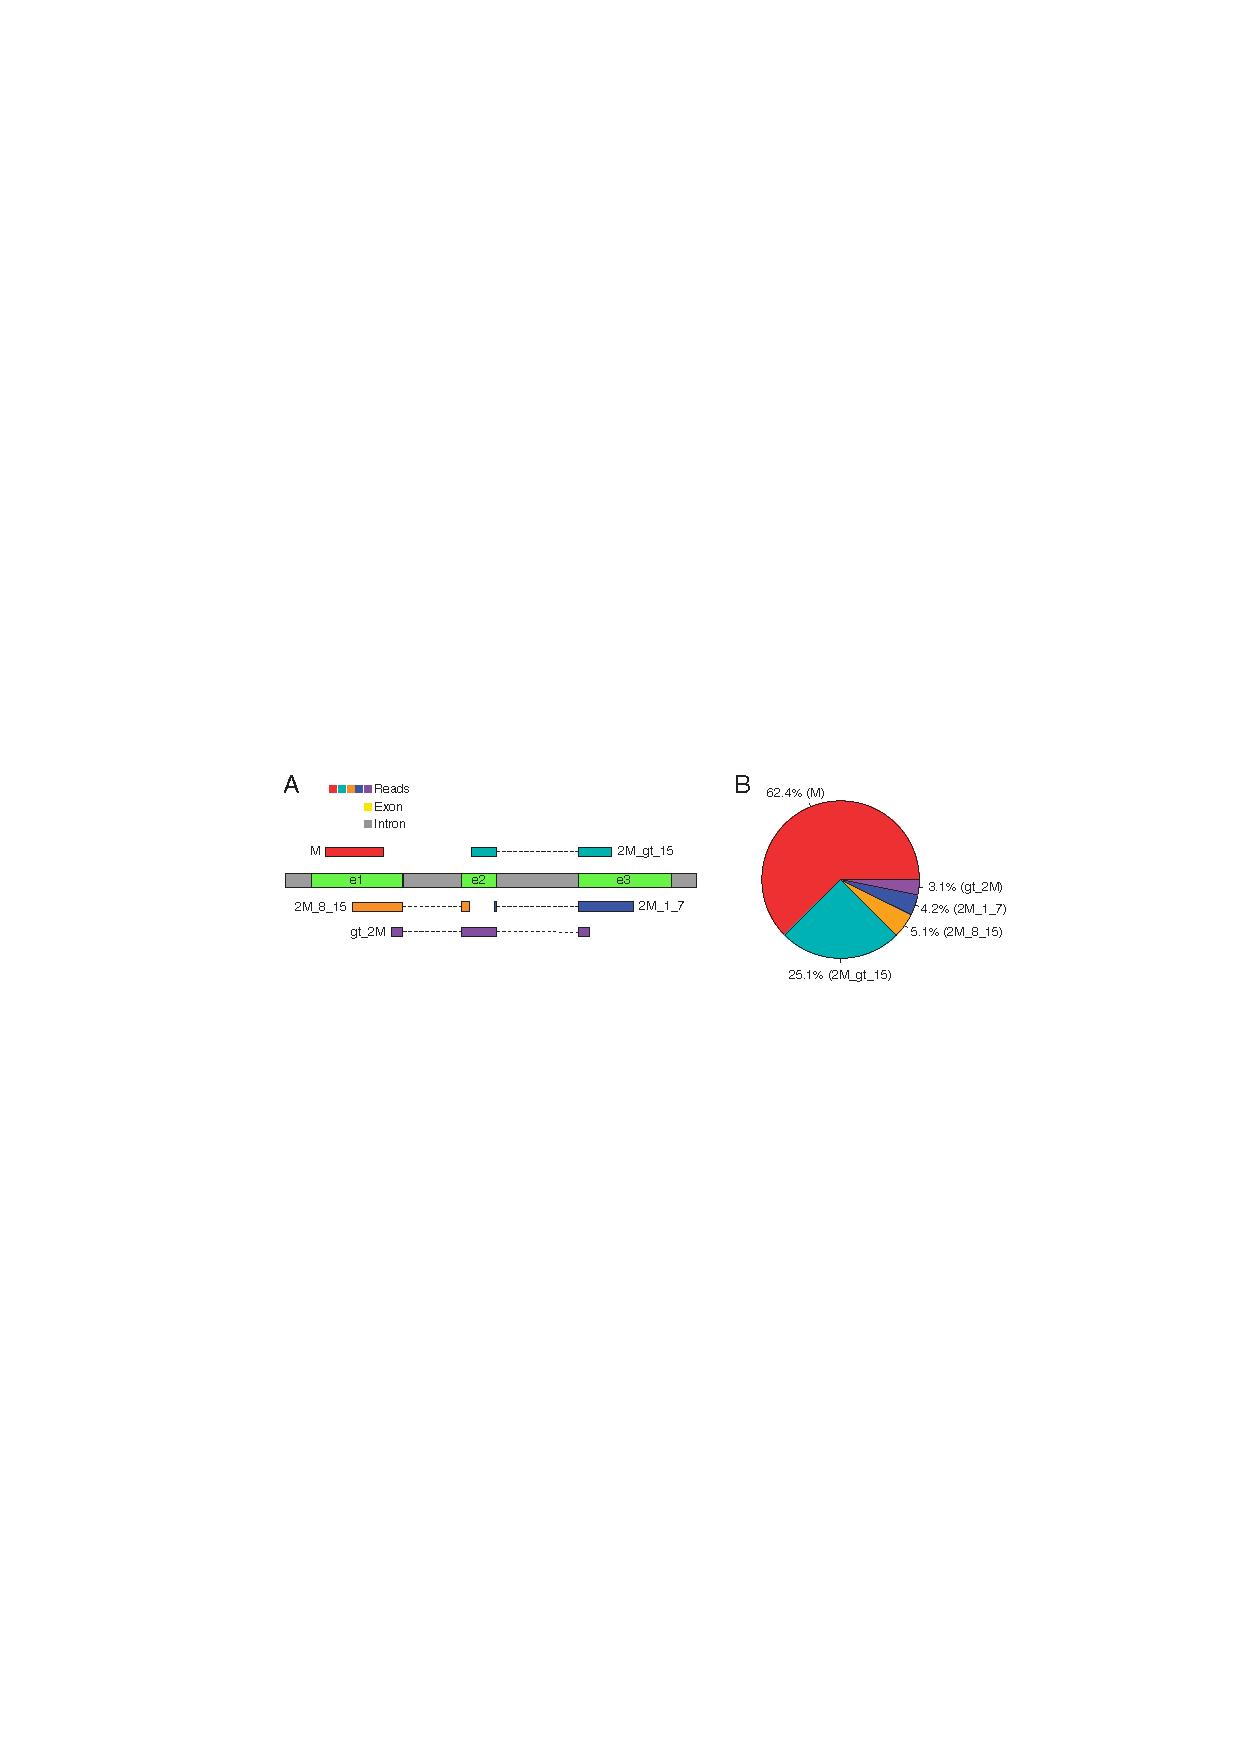
\includegraphics[width=1\linewidth]{img/chapter1/spliced_read_classes}
	  \caption[Read composition of an RNA-seq experiment]{\textbf{Read composition of an RNA-seq experiment.} (A) \citeauthor{Kim2015} simulated 20 million 100bp-reads for the human transcriptome and stratified the read set into 5 classes: (1) M, exonic read; (2) 2M\_gt\_15, junction reads with long, $>$15-bp anchors in both exons;
(3) 2M\_8\_15, junction reads with intermediate, 8- to 15-bp anchors; (4) 2M\_1\_7, junction reads with short, 1- to 7-bp, anchors; and (5) gt\_2M, junction reads spanning more than two exons. (B) Relative proportions of the read classes in the simulated dataset (Figure taken from \citeauthor{Kim2015} \citep{Kim2015}).}
	 \label{fig:splice_read_classes}
\end{figure}

First strategies to tackle this problem have been to transfer genome mapping methods and augment them with procedures to allow for splice-site detection. TopHat \citep{Trapnell2009} for example maps all reads against the genome using Bowtie \citep{Langmead}, and in a second step splits the unmapped read proportion into smaller segments to align them independently and searches the surrounding regions of the mapped segments for putative spliced connections. Other tools adopted the \textit{seed-and-extend} strategy such as GSNAP \citep{Wu2010} which splits reads into seeds to place them on the genome to narrow down the putative alignment regions to evaluate. The candidate regions are then evaluated by iteratively extending and merging of the initial seeds to determine the final alignment. All these early attempts at solving the spliced-read mapping problem in practice proved to be extremely time-consuming with run-times of several days for a single RNA-seq experiment, making them unsuitable for routine analysis of large scale transcriptomic datasets such as the ENCODE project \citep{Djebali2012} with several billions of short-reads \citep{Dobin2013}. In the following paragraphs, we discuss alternative strategies that have been developed and implemented in the currently most widely adopted spliced-read alignment tools to address the challenges of RNA-seq datasets.

\paragraph{Seed and cluster/stitch/score:} The central idea of \textit{seed} and \textit{cluster/stitch/score} extends the already presented \textit{seed-and-extend} paradigm from general-purpose read mappers by the concept of aligning reads directly to non-contiguous sequences via a Maximal Mappable Prefix (\textit{MMP}) search as implemented in STAR \citep{Dobin2013}. An $MMP$ can be seen as a contiguous part of the transcript as it is present in exons in the reference genome: Let $R$ be a read sequence, $G$ a reference genome sequence and $i$ a read location, then $MMP(R,i,G)$ is the longest substring ($R_i ... R_{i+MML-1}$) that matches one or multiple substrings in $G$ with $MML$ being the maximum mappable length. Finding seed matches of a read across multiple exons now becomes a sequential search of $MMP$s of the remaining unmapped portions of a read, until the entire read has been mapped as shown in Figure \ref{fig:star}.

\begin{figure}[h]
	 \centering
	 \includegraphics[width=0.7\linewidth]{img/chapter1/STAR}
	  \caption[The $MMP$ search as implemented by STAR]{\textbf{The $MMP$ search as implemented by STAR.} For an example read spanning two exons, in the first search step the $MMP$ 1 mapping to exon 1 is identified via a binary suffix array search. The next $MMP$ search is now performed on the remaining unmapped read proportion mapping to exon 2 (Figure adapted from \citeauthor{Dobin2013} \citep{Dobin2013}).}
	 \label{fig:star}
\end{figure}

This sequential search of unmapped read proportions for $MMP$s makes STAR very fast compared to the presented conventional reference-based read mapping algorithms and as a more natural approach to finding splice-junction matches is superior to arbitrary split-read methods such as TopHat or Bowtie. Technically, the $MMP$ search is implemented through uncompressed suffix arrays which allows for both a very fast search due to its logarithmic scaling and also has the $MMP$ search as direct consequence of the standard binary search without added computational effort \citep{Dobin2013}. In practice, this translates into a $>$ 50-fold speedup over conventional mappers. \\
Following the initial \textit{seed} step via the $MMP$ search, STAR builds the alignment of the entire read sequence in the \textit{cluster/stitch/score} step. In a first \textit{cluster} phase, all seeds are clustered by proximity to anchor seeds where anchor seeds represent seeds that map less than a user defined value. In the following \textit{stitching} phase, all seeds within defined windows are stitched together, following the assumption of a linear, local transcription model that disallows overlapping alignment blocks and enforces that the order of blocks identified in the reads is also maintained in the genome. In the final \textit{scoring} phase, the alignment score is calculated by a modified local alignment scheme. \\
It is important to note, that the apparent speed advantage of STAR comes at a significant tradeoff in terms of memory usage, since suffix arrays are space-wise very expensive: Compared to the BWT-based indices employed by TopHat of $\sim$4 GB for the human genome, STAR requires $\sim$27 GB of memory, therefore demanding dedicated high-memory compute nodes to load such indices (which however most research institutions have access to) \citep{Dobin2013}.

\paragraph{Hierarchical indexing for spliced alignment of transcripts:} This BWT-based strategy is implemented in HISAT \citep{Kim2015} with the main focus to reduce memory requirements and makes use of the fact that over 90\% of annotated introns in human are contained within a genomic interval of 64 kb. Mapping reads contained entirely within an exon or with two long anchors on either side, as shown in Figure \ref{fig:splice_read_classes}, can be usually mapped to a unique location. Spliced-read mapping becomes problematic, if one anchor is very short (8 - 15 bp), as matching such short anchors is computationally very expensive (8-bp occur statistically $\sim$48,000 times in the genome) and causes a lot of jumps and cache misses in a global FM-index \citep{Kim2015} during the search. HISAT addresses this via hierarchical indexing with two types of indices: (1) a global index containing the entire reference genome and (ii) a multitude of local indices that cover the genome, each index spanning 64 kb. In case of the human genome, this results in 48,000 local indices overlapping by 1,024 bp with its local neighbor which usually occupies only 4 GB of space since local indices are stored in small filesets. With such an indexing strategy at hand, one can map the longer read part in a \textit{global search} step and then by retrieving the corresponding local index usually map the remaining small anchor. This \textit{local search} is much faster due to the smaller local index size (typically 24 KB) which fits in cache in its entirety, therefore causing fewer cache misses. To speed up the search even faster, HISAT uses a direct read and reference sequence comparison for alignment extension once the genomic location of a read has been narrowed down. This requires the entire reference sequence in memory which in case of the human genome requires 682 MB \citep{Kim2015}. An example scenario of HISAT-based read mapping (in this case error-free reads) is illustrated in Figure \ref{fig:hisat}. With this hierarchical indexing strategy, HISAT allows for spliced-read mapping 10-100x faster than the naive spliced-read mappers TopHat and GSNAP while at the same time being very memory-efficient with a total of $\sim$4 GB of memory usage.

\begin{figure}[h]
	 \centering
	 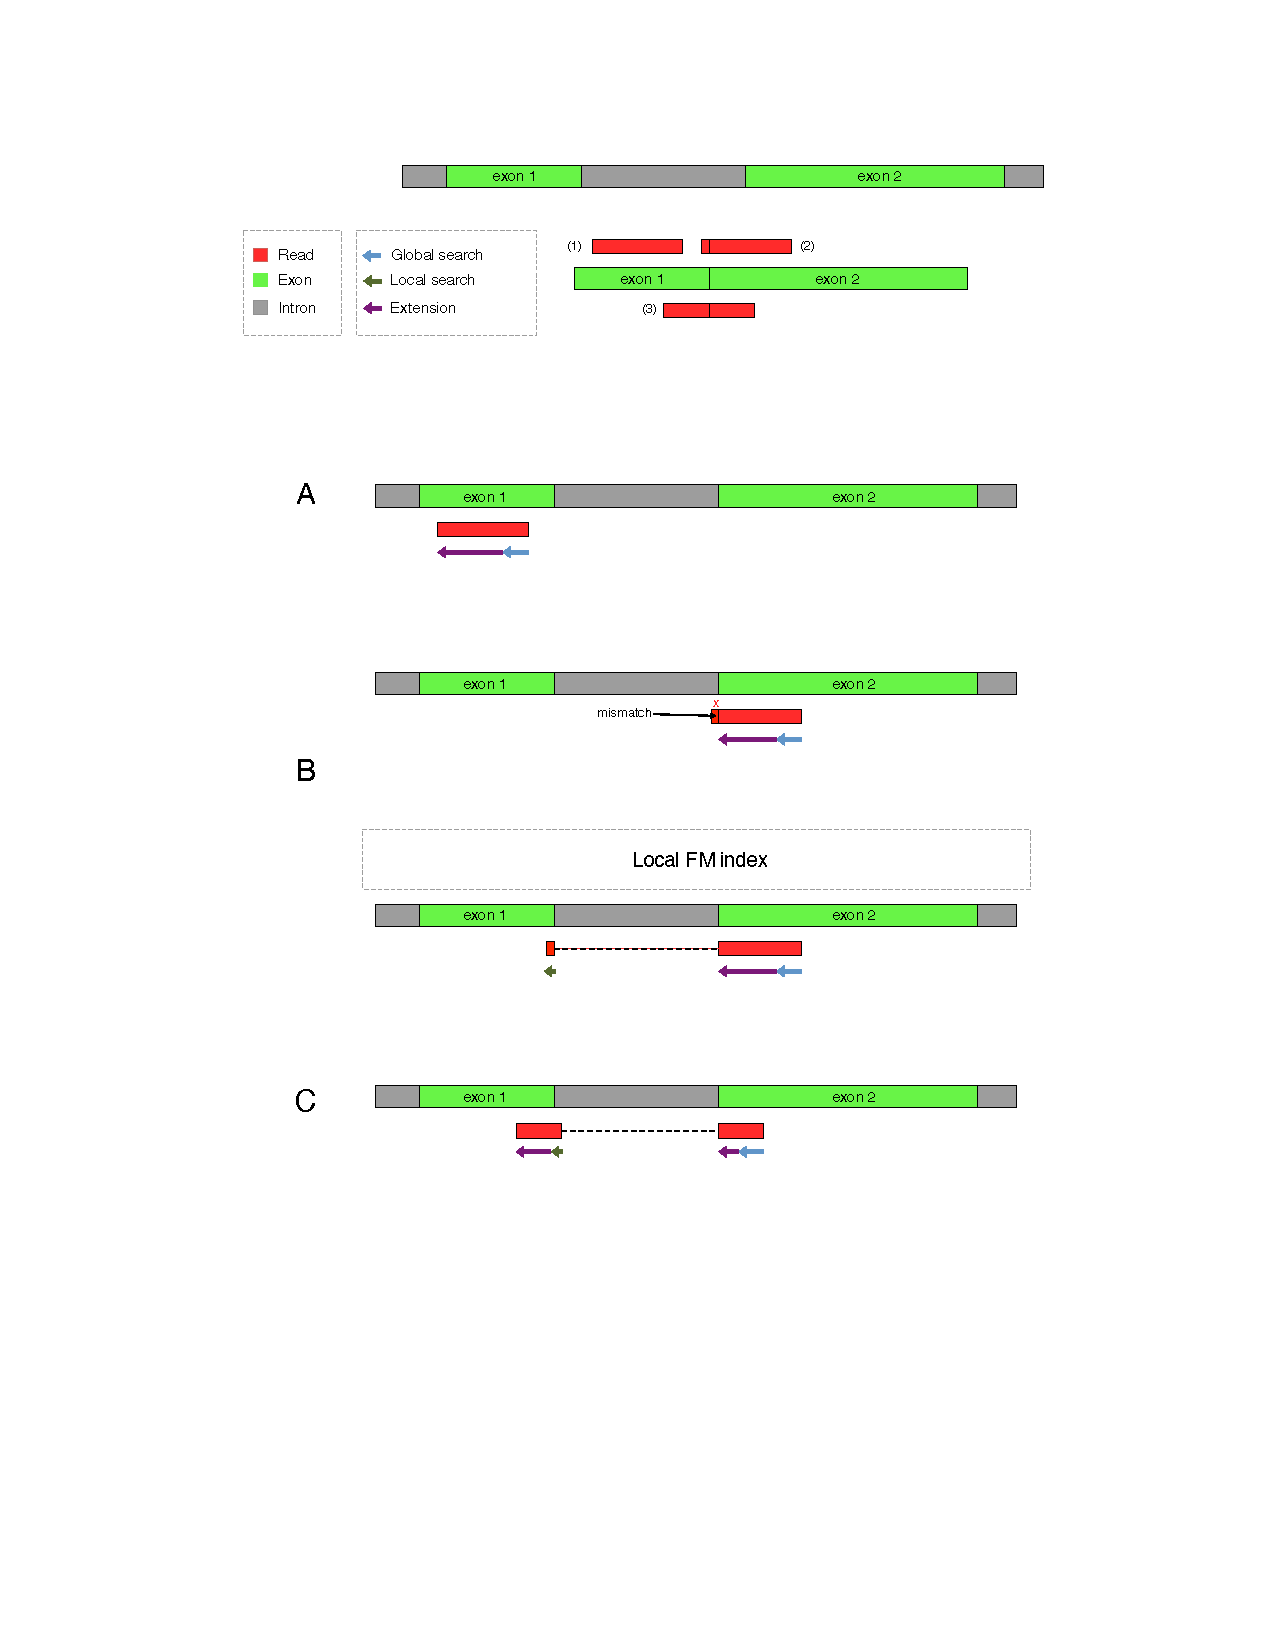
\includegraphics[width=1\linewidth]{img/chapter1/hisat}
	  \caption[Hierarchical indexing search example via HISAT]{\textbf{Hierarchical indexing search example via HISAT.} Three types of reads derived from a mature spliced-transcript are mapped: (1) a read contained within an exon, (2) a read spanning a splice junction with a short anchor and (3) a read spanning a splice-junction with long anchors. (A) Both read (1) and read (2) are initially mapped via the global index and after a 28 bp unique match HISAT switches to the extension step comparing base by base the remaining read and reference sequence. Read (1) matches till the end, for read (2) the extension stops after a mismatch close to the read end. (B) The corresponding local index is loaded where we search for the remaining bases of read (2) which are typically uniquely identified in a given local index and after checking for alignment compatibility, the spliced alignment for read (2) is reported. (C) For read (3), we again apply a mix of global search and extension until we hit a mismatch for the first anchor. Next, we load the local index that allows to quickly identify a unique mapping position for the second anchor before we switch to the extension mode to align the remaining part of the read (Figure adapted from \citeauthor{Kim2015} \citep{Kim2015}).}
	 \label{fig:hisat}
\end{figure}

\clearpage

\subsection{Mapping of nucleotide conversion containing reads}

Techniques employing conversion of nucleotides that are read out as mismatches during sequencing pose an additional challenge to existing reference-based read mapping approaches. The conventional approaches presented in earlier sections would treat those nucleotide conversions as mismatches, resulting in incorrect read alignments or failing to align such reads altogether, leading to substantial biases in the read out including a complete loss of signal for lowly expressed genes \citep{Zhang2021}. Because of the only very recent emergence of metabolic labelling methods, efforts have almost exclusively focused on the problem of processing bisulfite sequencing (BS-seq) derived reads, a method used to interrogate DNA methylation in genomic DNA that has been around considerably longer \citep{Frommer1992}. By applying bisulfite treatment followed by PCR amplification, unmethylated Cs are converted to Ts, leaving methylated Cs and all As, Ts and Gs unaffected as also illustrated in the top panel of Figure \ref{fig:3n}. In general, the C$>$T conversion rates are very high in such datasets, as methylation rates range from 0.1\% in \textit{Drosophila melanogaster} to $\sim$2-10\% in mammals \citep{Katoh2006} and the chemical conversion is highly efficient at $>$98\% \citep{Edelheit2013}. Two alternative approaches have been established to process such datasets: (1) Reduction of the four base alphabet to three letters (2) expansion of the search space by exploiting \textit{a priori} knowledge of what nucleotide conversion type is expected to occur during the conversion process.

\begin{figure}[h]
	 \centering
	 \includegraphics[width=1.0\linewidth]{img/chapter1/3N}
	  \caption[3N alignment as applied to bisulfite sequencing datasets]{\textbf{3N alignment as applied to bisulfite sequencing datasets.} Unmethylated Cs are converted to Ts during the bisulfite conversion step. In the forward strand version of the resulting sequencing read, all Cs are converted into Ts and in the reverse  strand version, all Gs are converted to As (equivalent to a T$>$C conversion on the reverse strand). Both read versions are aligned to the correspondingly converted reference sequence versions, resulting in a total of four alignment modes. Finally, from the four parallel alignment processes, the unique best alignment is determined (Figure adapted from \citeauthor{Krueger2011} \citep{Krueger2011}).}
	 \label{fig:3n}
\end{figure}

\paragraph{Three-nucleotide (3N) alignment:} The general idea of 3N-alignment is to assume all Cs in the reference have been converted - a reasonable assumption given the high conversion rates of bisulfite sequencing - and mask the distinction of detecting converted and unconverted bases by reducing the four letter base-space to a three letter base-space. This approach has been first implemented by BS Seeker \citep{Chen2010} and since then formed the center of the most popular BS-seq analysis tool Bismark \citep{Krueger2011} and as optional modes for general purpose alignment tools such as GSNAP. The central idea underlying all these approaches is illustrated in Figure \ref{fig:3n}: Both in the reads and the reference, all Cs are assumed to be unmethylated and thus converted from C$>$T (G$>$A as reverse stranded equivalent). Now standard tools are applied for the four different alignment modes: (1) Forward-converted read vs forward-converted genome, (2) forward-converted read vs reverse-converted genome, (3) reverse-converted read vs forward-converted genome and (4) reverse-converted read vs reverse-converted genome. From the four alignment modes, the best unique alignment is determined and reported per read. The reduction of the alphabet to three letters and subsequent loss of sequence complexity is also the most severe drawback of this approach, resulting in many more ambiguously mapped reads which cannot be uniquely placed anymore and for which randomly selected alignments are reported \citep{Zhang2021}. A more technical downside is the increased runtime due to the four alignment modes and the increase in memory by requiring a converted forward and reverse index. During the course of this thesis after finishing the SLAM-DUNK package featured in chapter \ref{chap:slamdunk}, we made Daehwan Kim, project leader of TopHat2, HISAT and HISAT2, aware of the SLAM-seq technology harnessing T$>$C conversions which prompted the development of HISAT-3N \citep{Zhang2021}. HISAT-3N generalizes the 3N alignment from a rigid bisulfite conversion model to any configurable type of base conversion, using HISAT2 as underlying alignment engine, therefore also allowing for spliced-read alignment required for RNA-seq data analysis. Likewise, the bisulfite RNA-seq toolkit meRanTK \citep{Rieder2016} adopted the 3N-alignment approach using STAR as alignment engine to process bisulfite RNA-seq datasets.

\paragraph{Enumeration and asymmetric scoring:} In contrast to reducing the base alphabet, enumeration approaches using hash-based seeding make use of the fact that with a single expected conversion-type, it is possible to enumerate all possible converted states of a $k$-mer in the reference sequence (given a sufficiently small $k$). This enumeration approach to create a hash table of seeds is both implemented e.g. by BSMAP \citep{Xi2009} and BiSS \citep{Dinh2012AdvancedArabidopsis} and restores the 1-to-1 correspondence between a $k$-mer in the read and reference, allowing now again the candidate position retrieval from a hash table lookup despite the present bisulfite conversions as illustrated in Figure \ref{fig:bisulfitehash}.

\begin{figure}[h]
	 \centering
	 \includegraphics[width=0.7\linewidth]{img/chapter1/bisulfite_enumeration}
	  \caption[Enumeration of bisulfite conversions seed hash table]{\textbf{Enumeration of bisulfite conversions seed hash table.} Seeds are created from the reference at a fixed length $k$. For each original seed, all possible bisulfite converted versions of the original seed are enumerated and added to the hash lookup table. Using this extended seed hash table, seeds from bisulfite converted reads can be directly looked up in a conventional manner without additional read conversion steps (Figure adapted from \citeauthor{Xi2009} \citep{Xi2009}).}
	 \label{fig:bisulfitehash}
\end{figure}

After determining the candidate regions, BSMAP converts the Ts to Cs in the read sequence at reference Cs and uses a hamming-distance based approach to calculate the alignment scores. BiSS uses NextGenMap \citep{Sedlazeck2013} as alignment engine and applies a custom scoring matrix as shown in Table \ref{tab:bissscoring} to the Smith-Waterman alignment function. The scoring matrix is tailored to the asymmetry of the C$>$T conversions occurring during bisulfite treatment and treats C$>$T and G$>$A (reverse strand C$>$T) as a match.

\begin{table}[!ht]
\begin{center}
\begin{footnotesize}
\noindent\makebox[\textwidth]{%
\begin{tabular}{c|rrrr}\hline
 &\textbf{A} & \textbf{G} & \textbf{C} &\textbf{T} \\\hline
\textbf{A} &4&-2&-2&-2 \\%\hline
\textbf{G} &\textbf{4}&4&-2&-2 \\%\hline
\textbf{C} &-2&-2&4&\textbf{4} \\%\hline
\textbf{T} &-2&-2&-2&4 \\\hline
\end{tabular}}
\end{footnotesize}
\end{center}
\caption[Asymmetric scoring matrix for bisulfite conversions as implemented in BiSS]{\textbf{Asymmetric scoring matrix for bisulfite conversions as implemented in BiSS.} In addition to base identity treated as a match with a score of 4, also C$>$T and G$>$A (reverse complement C$>$T) are treated as matches with a score of 4 since these conversion occur during bisulfite treatment. All other combinations are treated as mismatches and penalized with -2.}
\label{tab:bissscoring}
\end{table}

Compared to 3N-approaches, enumeration and asymmetric scoring methods achieve a higher sensitivity as shown in numerous studies \citep{Chatterjee2012,Harris2010,Zhang2021,Dinh2012AdvancedArabidopsis} with little overhead in terms of compute time or memory consumption.

\clearpage

\section{Simulations to evaluate bioinformatics methods}

Simulations imitate the behavior of a real-world process or system over time \citep{Banks2004DiscreteEvent}. In the field of computer science, a computer simulation attempts to model a real-life or hypothetical situation \textit{in silico} to study how the system works. In the scope of a simulation, the model contains the key parameters and behaviors of the system or process under investigation and the simulation refers to the evolution of this model over time. Typically, simulations are used when the real system cannot be engaged, is too dangerous, too costly to perform real-world experiments or too complex for analytical solutions \citep{nla.cat-vn3969224}. In the context of next-generation sequencing, computational methods can be evaluated using empirical or simulated data. Benchmarking with real empirical datasets is crucial to evaluate the overall validity of the benchmarked methods in a real-world scenario. The main disadvantage is that the underlying truth is not known, therefore a detailled evaluation of the accuracy is impossible \citep{Escalona2016}. Simulation \textit{in silico} is the commonly used complementary method, as this allows for an in depth analysis of all aspects of the simulated process and all methods under investigation can be thoroughly benchmarked against the true values from the simulation. In contrast to costly and slow-turnover real-world experiments, simulations allow for a much quicker development cycle of new methods \citep{Zhao2017} and have been used as guidance for the development of new computational tools \citep{Huang2012}, generally debugging and software performance evaluation \citep{Hu2012,Caboche2014}, as well as hypothesis generation \citep{Hoban2012} and to aid the design of sequencing projects \citep{Shendure2012,Shcherbina2014}. In this section, we will focus on the characteristics of current methods to simulate next-generation sequencing reads and simulation frameworks for RNA-seq processes and comment on their suitability to ultimately benchmark existing methods for the analysis of epitranscriptomics datasets.

\subsection{Simulation of next-generation sequencing reads}

There are a number of sequencing platform technologies currently on the market such as Illumina's sequencing by synthesis (the most widely adopted platform for RNA-seq), pyrosequencing as employed by Roche's 454 platform, semiconductor sequencing by Thermo Fisher's IonTorrent, or the newer long-read sequencing platforms Pacific Biosciences' (PacBio) single-molecule, real-time (SMRT) sequencing and Nanopore sequencing as performed on Oxford Nanopore Technologies' platform. Each of these platforms produces reads with different characteristics such as read length, (ranging from $<$75bp to several kb) or read type (single- or paired-end) and produces these reads with different error profiles. A general overview of sequencing platforms is provided by \citeauthor{Liu2012} \citep{Liu2012}. Independent of the platform under investigation, next-generation sequencing read simulators base their simulations on several key parameter sets (see Figure \ref{fig:simulator_overview}):

\begin{figure}[h]
	 \centering
	 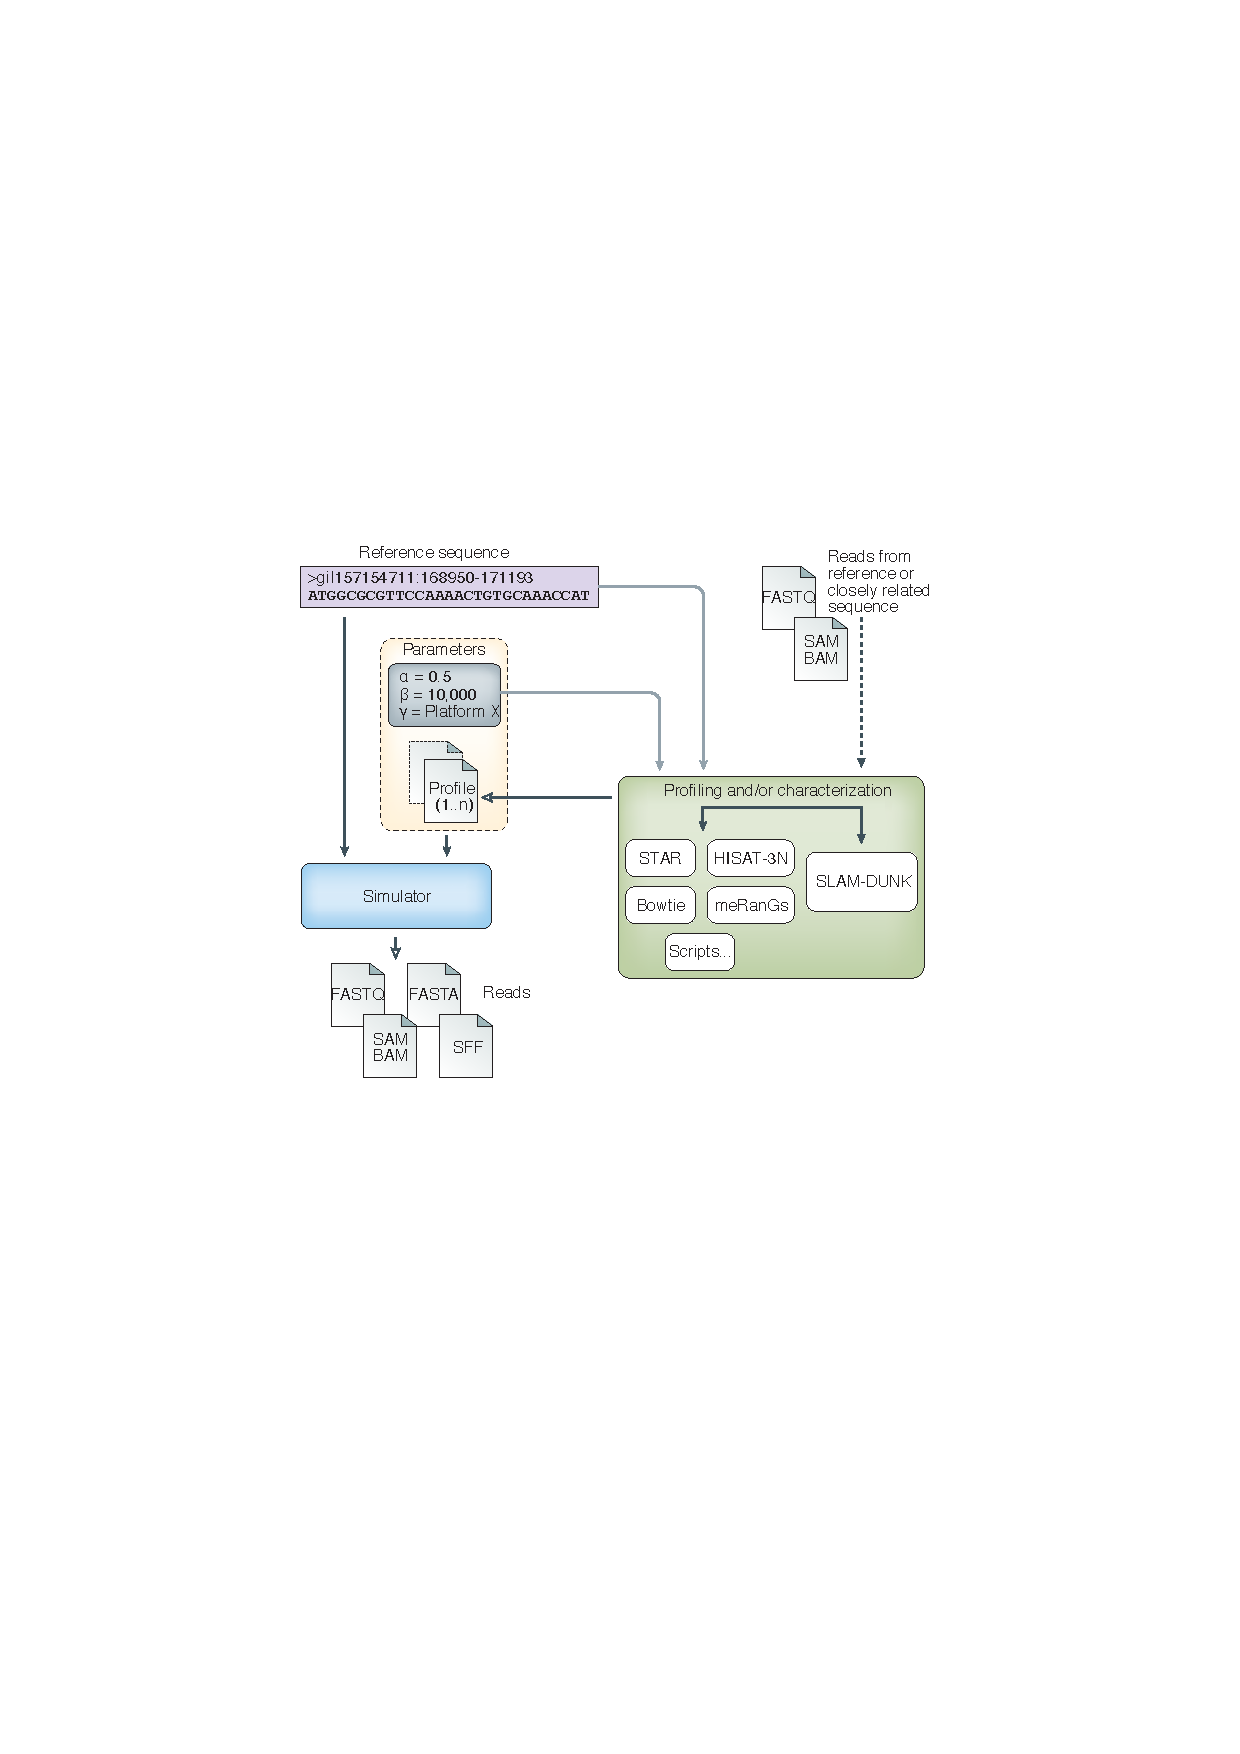
\includegraphics[width=0.7\linewidth]{img/chapter1/simulator_overview}
	  \caption[Generalized NGS simulation overview]{\textbf{Generalized NGS simulation overview.} A simulation process requires as input (usually) a reference sequence and the simulation parameters. Part of the parameters that relate to e.g. platform specific error profiles are in some cases directly estimated from empirical datasets. The output of the simulator is then the simulated reads (with or without quality information) or alignments with the encoded truth values in different formats. (Figure adapted from \citeauthor{Escalona2016} \citep{Escalona2016}).}
	 \label{fig:simulator_overview}
\end{figure}

\paragraph{Reference sequence:} The simulation needs a reference sequence as template to simulate reads from. Most read simulators use haploid sequences as reference, some simulators such as pIRS \citep{Hu2012}, ReadSim \citep{Lee006395} and SimSeq \citep{Earl2011} allow for simulation from different ploidy levels or even metagenomic abundance profiles. The XS read simulator \citep{Pratas2014} on the other hand simulates reads with random nucleotides given the read length, sequencing technology and nucleotide composition.

\paragraph{Read numbers:} The sequencing machine determines the type of reads it can produce in terms of length or read type and overall read numbers. Therefore, these are also important parameters for the simulator to take into account. Most simulators allow to specify the overall coverage of the reference sequence, which will be directly translated into read numbers produced by the simulator. Since DNA amplification is a crucial step in many library preparation protocols, it is also often desired to evalate the bias introduced by PCR. Read simulators such as ART \citep{Huang2012} simulate PCR bias via the read number per amplicon parameter \citep{Mardis2008}. A more sophisticated PCR bias implementation is done by e.g. Grinder \citep{Angly2012} which simulates amplicon sequencing from a user-supplied PCR primer collection and therefore can also evaluate experimental artifacts such as chimeras \citep{Haas2011} and spurious copy number variants \citep{Escalona2016}. Other simulators like pIRS simulate the bias introduced during PCR amplification by taking the underlying GC-content of the regions of interest into account. 

\paragraph{Error models:} Different platforms produce different error types at different rates. In a simulation, these errors are introduced via error-rate models that determine for a given read position the probability of an erroneous substitution or indel \citep{Escalona2016}. Indels have been reported to be very rare on the Illumina platforms, but in contrast being the main error source on the 454 and IonTorrent \citep{Dohm2008}, as well as the PacBio \citep{Loman2012} and Nanopore platform \citep{Ono2013}. Substitution errors on the other hand are the dominant error source on the Illumina sequencing platform \citep{Hu2012} and are position specific with higher error rates in later sequencing cycles \citep{Metzker2010SequencingGeneration}. Without in-depth knowledge of the platform and its biases, it is very difficult to come up with reasonable parameter values for the majority of the users. Therefore, many simulators provide default profiles or alternatively, provide tools that allow the estimation of error profiles \textit{de novo} from empirical datasets. Simulators such as pIRS provide a full framework to use alignment tools such as Bowtie or BWA in combination with error estimation software such as DRISEE \citep{Keegan2012} to extract custom error profiles. ART and pIRS on the other hand generate quality profiles based on error models that are derived from their own empirical datasets.

\paragraph{Quality scores:} Quality scores are reported by the sequencing machine during basecalling and are a proxy for the probability of an error in a base call \citep{Ewing1998,Ewing1998a}. Quality scores are typically position dependent, with the average quality score decreasing with increasing base positions for most sequencing technologies \citep{Huang2012}. Simulators like Flowsim \citep{Balzer2010} use predefined quality score profiles based on previous studies. Other simulators like ART again provide tools to allow the user to derive custom quality score models from FASTQ files directly. Conversely, simulators like XS simply use a fixed quality score for every read. More complex simulation as done by Mason \citep{Holtgrewe2010} use a position-specific normal distribution and define the mean, standard deviation and quality standard deviation for both the 5' and 3' end of the read. For long reads, where the error distribution is assumed to be constant, simulators such as pbsim \citep{Ono2013} assume a uniform distribution of quality scores.

\paragraph{Genomic variants:} On top of sequencing errors, genomic variants also introduce variability in the derived simulated read sets. In general, genomic variants such as SNPs, indels, inversions, translocations and CNVs are already introduced in the reference sequence before starting the read simulation \citep{Pattnaik2014}. These variants can be either introduced at a predefined mutation rate, or supplied via a file of known mutations (such as contained in a VCF file). Other programs like Mason can generate related haplotype sets differing by at least one mutation from the reference sequence. 

\paragraph{Read output:} The simulated reads sets are typically stored in the platform specific output formats like SFF for 454 files or FASTQ files for the IonTorrent, Illumina, PacBio and Oxford Nanopore platform. Some simulators like ART, Mason or pbsim also produce alignment files in the common MAF, SAM and BAM formats.
\\ 

A thorough and comprehensive overview of the state-of-the-art landscape of next-generation sequencing read simulators and guidelines how to choose among them is provided by \citeauthor{Escalona2016} \citep{Escalona2016} and \citeauthor{Zhao2017} \citep{Zhao2017} and reports ART \citep{Huang2012} as the best supported general purpose read simulator for the Illumina sequencing platform. Notably, while there exist simulators to mimic bisulfite sequencing such as the WGBSSuite \citep{Rackham2015}, none of the reported sequencing read simulators allow for the simulation of nucleotide conversion processes such as employed by epitranscriptomics sequencing methods.

\subsection{Simulation of RNA-seq processes}

The ideal scenario to characterize the true full transcriptome in a real experiment is not feasible with current techonologies, therefore scientists resort to simulation software as a proxy for benchmarking RNA-seq analyis methods. Compared to plain next-generation sequencing read simulators, there are several added layers of complexities that have to be modelled by an RNA-seq simulator. As a first \textit{biological layer}, a gene can have multiple transcript variants in different splicing states and abundances, which needs to be factored in a model to deduce which transcript sequence to use (isoform), what type of reads (unspliced from pre-mRNA or spliced from mature mRNA) and how many reads (transcript abundance) to simulate (see Figure \ref{fig:rnaseq_simulator_layers} top panel). Once we have determined a realistic transcript pool, there is a second \textit{technical layer} of RNA library preparation steps that have to be accounted for (Figure \ref{fig:rnaseq_simulator_layers} bottom panel). These steps include reverse transcription, fragmentation, adapter ligation, amplification via PCR, and finally sequencing, each of them potentially introducing biases \citep{Sendler2011,Hansen2010,Benjamini2012}. Several RNA-seq simulators have been published at this point that predominantly focus on either the biological or the technical layer which are discussed in this section.

\begin{figure}[h]
	 \centering
	 \includegraphics[width=1.0\linewidth]{img/chapter1/rnaseq_simulation-block_diagram}
	  \caption[Layers to address by an RNA-seq simulator]{\textbf{Layers to address by an RNA-seq simulator.} The biological layer contains all processes and variables contributing to the overall complexity of RNA molecules in the transcript pool to be sequenced. These include potentially multiple splice variants per genes at different abundance levels and in different splicing states. The technical layer comprises all the experimental steps taken in the wetlab to proceed from isolated RNA to a final RNA-seq library that is ready to be sequenced.}
	 \label{fig:rnaseq_simulator_layers}
\end{figure}

\paragraph{Biological layer:} Technical simulators such as Flux \citep{Griebel2012} and rlsim \citep{https://doi.org/10.48550/arxiv.1308.3172} randomly assign expression values to transcripts from a parametric distribution. A straightforward approach to simulate more realistic transcript abundances is proposed by RSEM \citep{Li2011}, which uses real RNA-seq datasets to map them with the conventional read mapper Bowtie against annotated transcript sequences to deduce an empirical gene expression model. However, the model is dependent on the provided annotation and data and does not account for alternative or partial splicing events. This additional complexity is tackled by BEERS \citep{Grant2011} that builds consensus gene models from 11 annotations and simulates alternative-splicing events by randomly removing exons at a given rate. As BEERS introduces such alternative splicing events by chance, there is no control over the number, distribution or types of the events. Similar to RSEM, BEERS deduces realistic gene abundance values from real datasets as input. ASimulatoR \citep{Manz2021} set out to improve the user's control over the distribution and type of alternative splicing events by collecting all exons per gene to serve as unspliced templates. From those templates, all possible combinations of 8 types of alternative-splicing events are created and the user can specify the number of genes and type of events to include in the simulation which are again produced at a given rate. While ASimulatoR gives the user more control over the observed splice-variants, it does not support the definition of custom splicing states of transcripts at fine granularities to e.g. dissect splicing kinetics. CAMPAREE \citep{Lahens2021} attempts to address these issues by simulating RNAs at molecule level and trying to capture all the different states of transcription, editing, splicing and degradation. Like other tools, CAMPAREE uses real datasets to estimate intron and exon abundance distributions. This data is aggregated at transcript- and gene-level to obtain transcript and gene abundance distributions. Molecules are then simulated by randomly selecting an isoform for a gene according to its abundance distribution and calculating the likelihood of it being an unspliced pre-mRNA precursor by looking at the ratio of intronic reads per base. The transcript sequences are mapped back to the reference sequence and reported in FASTA format. CAMPAREE allows for the distinction of fully unspliced pre-mRNA and spliced mature RNA, but there is no indicated support for partially spliced transcripts required to simulate splicing kinetics. \textit{Polyester} \citep{Frazee2015} on the other hand takes a different path and focuses on the ability to simulate reads at differential expression levels across biological replicates to evaluate differential expression analysis toolkits. Like the other discussed tools, \textit{Polyester} estimates expression values from public datasets and then simulates read counts per transcript following a negative binomial model at user defined differential expression levels per replicate. In addition to the simulated reads in FASTA format, a corresponding abundance matrix listing per transcript the differential expression status and fold change is reported.

\paragraph{Technical layer:} When it comes to the individual experimental steps performed during an RNA-seq experiment, the simulators focusing on the biological layer of establishing a realistic RNA pool typically put less effort into modelling of the experimental procedure: RSEM only models fragmentation, read length distributions, sequencing error and quality scores, all values extracted from real datasets. Likewise, BEERS models fragmentation and a user defined base error and a tail error. ASimulatoR uses a modified version of \textit{Polyester} as their read simulation engine that on top models PCR duplicates and adapter contamination for all fragments shorter than the supplied read length. CAMPAREE follows the same path and stops at outputting the transcript sequences, leaving the read simulation to other simulator engines. \textit{Polyester} employs a more sophisticated approach that approximates fragmentation with several models, allowing for a uniform fragmentation or a 3' end or center bias. Read error models are less sophisticated uniform error models based on user-defined values or values derived from empirical data. The Flux simulator was designed to specifically simulate all RNA-seq processes ranging from reverse transcription, fragmentation, adapter ligation, amplification via PCR, and sequencing. All experimental steps are sophistically modeled using empirical attributes derived from experiments, such as enzymatic specificity and activity during fragmentation, random hexamer priming and resulting priming collisions from multiple priming events during reverse transcription, adapter ligation efficiency using underlying motifs, GC-bias during PCR amplification and sequencing error models. Likewise, rlsim  models fragmentation, priming, PCR amplification and size selection with a particular focus on PCR and size selection steps on the Illumina platform.
\\

In summary, there is no identifiable RNA-seq simulator that excels both at the step of simulating a realistic pool of transcripts in different splicing-states, isoforms and abundances while modelling all the technical steps of getting from isolated RNA to sequencing reads from a preppred library. The most reasonable approach some simulators like ASimulator and CAMPAREE follow is to only focus on one layer - in their case the biological layer - and outsource the raw read simulation to other simulation frameworks. While some simulators generate splice-variants and mature and unspliced transcript forms, none of them allows for fine-granular control of the splicing states per intron to realistically simulate partially spliced transcripts as they are investigated during splicing kinetics analysis. Notably, also none of the RNA-seq simulators allow for simulation of nucleotide conversions from the epitranscriptomics sequencing toolbox.

%\paragraph{Polyester:} 
%
%\begin{itemize}
%	\item Its main advantage is the abil- ity to simulate reads indicating isoform-level differential expression across biological replicates for a variety of experimental designs
%	\item Polyester was created to fulfill the need for a tool to simulate RNA-seq reads for an experiment with replicates and well-defined differential expression.
%	\item Input FASTA or GTF
%	\item Parameters estimated from public datasets. 
%	\item Read counts negative binomial. The negative binomial model for read counts has been shown to satisfactorily cap- ture biological and technical variability (Anders and Huber, 2010; Robinson et al., 2010)
%	\item Library size factors + GC content models
%	\item Input custom read count matrices also possible
%	\item Model fragmentation with static mean/std or empirical, uniform fragments or 3' end or center bias
%	\item reads from both strands equally
%	\item Uniform or empirical error models
%	\item FASTA(!) + matrix transcript name, differential expression status and fold change is recorded. For each replicate, the file name, group identifier j and library size factor is recorded.
%\end{itemize}
%
%\paragraph{Flux simulator:}
%
%\begin{itemize}
%	\item Specifially designed to simulate experimental RNA-seq processes
%	\item Expression profile FASTA + GTF - randomly assigns expression value to transcript
%	\item Fragmentation (enzymatic specificity and activity)
%	\item RT - first strand synthesis, random hexamer priming events, multiple priming and collisions, second strand synthesis
%	\item Size selection
%	\item Adapter ligation (Motifs of adapter sequences)
%	\item PCR amplification (GC-content)
%	\item Sequencing error models
%\end{itemize}
%
% All of these ex- perimental steps are modeled using empirical attributes in an experimental protocol. This is useful for introducing the ap- proximate experimental biases for real RNA-seq. Furthermore, by comparing simulated read distributions with experimental evidence, the Flux Simulator supports four organisms (Saccharomyces cerevisiae, Arabidopsis thaliana, Mus musculus and Homo sapiens). However, it does not include the comprehensive transcription annotations. Rather, it uses only one representa- tive annotation for each organism such as SGD and TAIR for Saccharomyces cerevisiae and Arabidopsis, respectively, and RefSeq for both Mus musculus and Homo sapiens.
% 
% \paragraph{rlsim}
% 
% Similar to Flux Simulator, the rlsim tool was developed to simulate RNA-seq libraries with parameter estimation for the Illumina platform. The rlsim also mimics the major RNA-seq processes including fragmentation, priming, PCR amplification and size selection with a particular focus on PCR and size selec- tion steps. All these simulations estimate parameters for insert size, corrected and uncorrected relative expression levels and GC-dependent amplification efficiencies, which are inputted into a thermodynamic model of oligonucleotide hybridization to generate sample-specific data.
%
%\paragraph{RSEM:} The simulator included with RSEM develops an empirical model of gene expression by quantifying real RNA-Seq datasets and using the ex- pression parameters as the basis for simulation. 
%
%\paragraph{BEERS:} 
%
%\begin{itemize}
%	\item Alternative splicing
%	\item configurable rates for splice isoforms
%	\item quality values	
%	\item Gene models from 11 annotations
%	\item Filter for splice-site motifs
%	\item Randomly choose subset of gene models
%	\item To introduce an AS event, BEERS randomly removes exons from a gene. No control.
%	\item Measure alignment accuracy + splice site calling
%\end{itemize}
%
%\paragraph{ASimulatoR:} 
%
%\begin{itemize}
%	\item Alternative splicing
%	\item ASimulatoR collects all annotated exons from all transcript variants in the genome annotation and merges them in ‘exon supersets’ serving as unspliced templates.
%	\item ASimulatoR supports eight types of events: exon skipping, multiple exon skipping, intron retention, alternative 3’-splice site, alternative 5’-splice site, mutually exclusive exons, alternative first exon and last exon.
%	\item The user can define the number of overall genes in the simulated set and select AS event types to be included together with their distribution. 
%	\item Events produced at given rate.
%	\item Produced transcript variants serve as an input for RNA-Seq reads simulation.
%	\item Simulation with polyester + PCR duplicates + adapter contamination
%	\item Adapters added to fragments shorter than read lengths. Duplicates drawn from Poisson with lambda = 1
%	\item fastq + count file
%\end{itemize}
%
%\paragraph{Polyester:} 
%
%\begin{itemize}
%	\item Its main advantage is the abil- ity to simulate reads indicating isoform-level differential expression across biological replicates for a variety of experimental designs
%	\item Polyester was created to fulfill the need for a tool to simulate RNA-seq reads for an experiment with replicates and well-defined differential expression.
%	\item Input FASTA or GTF
%	\item Parameters estimated from public datasets. 
%	\item Read counts negative binomial. The negative binomial model for read counts has been shown to satisfactorily cap- ture biological and technical variability (Anders and Huber, 2010; Robinson et al., 2010)
%	\item Library size factors + GC content models
%	\item Input custom read count matrices also possible
%	\item Model fragmentation with static mean/std or empirical, uniform fragments or 3' end or center bias
%	\item reads from both strands equally
%	\item Uniform or empirical error models
%	\item FASTA(!) + matrix transcript name, differential expression status and fold change is recorded. For each replicate, the file name, group identifier j and library size factor is recorded.
%\end{itemize}
%
%\paragraph{Camparee:} 
%
%\begin{itemize}
%	\item molecule-level simula- tion of input RNA samples
%	\item These in- clude molecules produced from the same gene that are in different states of transcription, editing, splicing, and degradation [14–17].
%	\item The output of CAMPAREE is intended primarily to prime other RNA-Seq simulators, which will then model the biases introduced by library preparation and sequencing.
%	\item Input FASTA or GTF, optionally file indicating ploidy
%	\item FASTQ files or reads
%	\item Camparee estimates intron and exon abundance distributions from real data
%	\item Transcript-level read counts are aggregated into gene-level read counts for transcript and gene abundance distributions
%	\item Simulate molecules: 
%	\item 1) Ran- domly select a gene from the gene distribution. 3) Randomly select an isoform for this gene from the transcript distribution. 4) Randomly determine whether to generate an unspliced version of the transcript (i.e. pre-mRNA containing all introns) by calculating the likelihood of pre-mRNA as the ratio of intronic read counts per base (from the in- tron distribution) to the gene-level read counts per base. By using average read counts per base, this accounts for differences in length between a gene’s introns and exons. 5) Having selected which transcript to generate, retrieve the full nucleotide sequence for the transcript and gen- erate CIGAR strings mapping the transcripts back to the appropriate parental genome and the original reference genome. 6) Add a polyA tail to the 3 end of the se- quence and corresponding entries for soft-clipped bases (denoted by ‘S’) to the appropriate ends of each CIGAR string. Lastly, CAMPAREE saves this list of simulated molecules in either FASTA format, listing the full se- quence and identifier for each molecule, or in a tab- delimited “molecule file” that lists the molecule sequence along with other metadata, including the reference and parental CIGAR strings.
%\end{itemize}
